% ============================================================================
%  Methodology -- HyperAVNet.  Self-contained: % ============================================================================
%  Methodology -- HyperAVNet.  Self-contained: % ============================================================================
%  Methodology -- HyperAVNet.  Self-contained: % ============================================================================
%  Methodology -- HyperAVNet.  Self-contained: \input{sections/method} in any paper.
%  Requires: amsmath, amssymb, bm, booktabs, graphicx, (cleveref optional).
% ============================================================================
\section{Methodology}
\label{sec:method}

\subsection{Problem formulation}
\label{sec:problem}
Each sample of AV-FFIA is a synchronised two-second clip $(\mathbf{x}^{a}, \mathbf{X}^{v})$, where
$\mathbf{x}^{a}\in\mathbb{R}^{L}$ is the hydrophone waveform ($L = 2f_s$, $f_s = 64$\,kHz) and
$\mathbf{X}^{v}\in[0,1]^{3\times T\times H\times W}$ holds $T$ RGB frames sampled uniformly from the
overhead camera. The label $y\in\mathcal{Y}=\{\textsc{None},\textsc{Weak},\textsc{Medium},\textsc{Strong}\}$
is the feeding intensity. We learn $f_{\theta}:(\mathbf{x}^{a},\mathbf{X}^{v})\mapsto\mathbf{p}\in\Delta^{|\mathcal{Y}|-1}$ with
two goals that pull in opposite directions: high accuracy, robust to the acoustic and visual
corruptions typical of aquaculture (bubbles, pumps, low light, reflections), and a small
parameter and compute budget for on-site deployment.

HyperAVNet (Fig.~\ref{fig:overview}) has four parts. Two hypercomplex backbones map each modality to a
hierarchy of \emph{stage tokens} (Sec.~\ref{sec:backbones}). A set of shared \emph{bottleneck tokens}
is updated by hypercomplex component fusion (HCF) blocks attached at a configurable subset of
stages, with zero-initialised cross-modal feedback into both streams (Secs.~\ref{sec:hcf},~\ref{sec:schedule}).
Fused and unimodal heads produce the predictions (Sec.~\ref{sec:heads}). The model is trained with a
multi-level distillation objective from a pretrained audio-visual teacher (Sec.~\ref{sec:objective}).

\begin{figure*}[t]
  \centering
  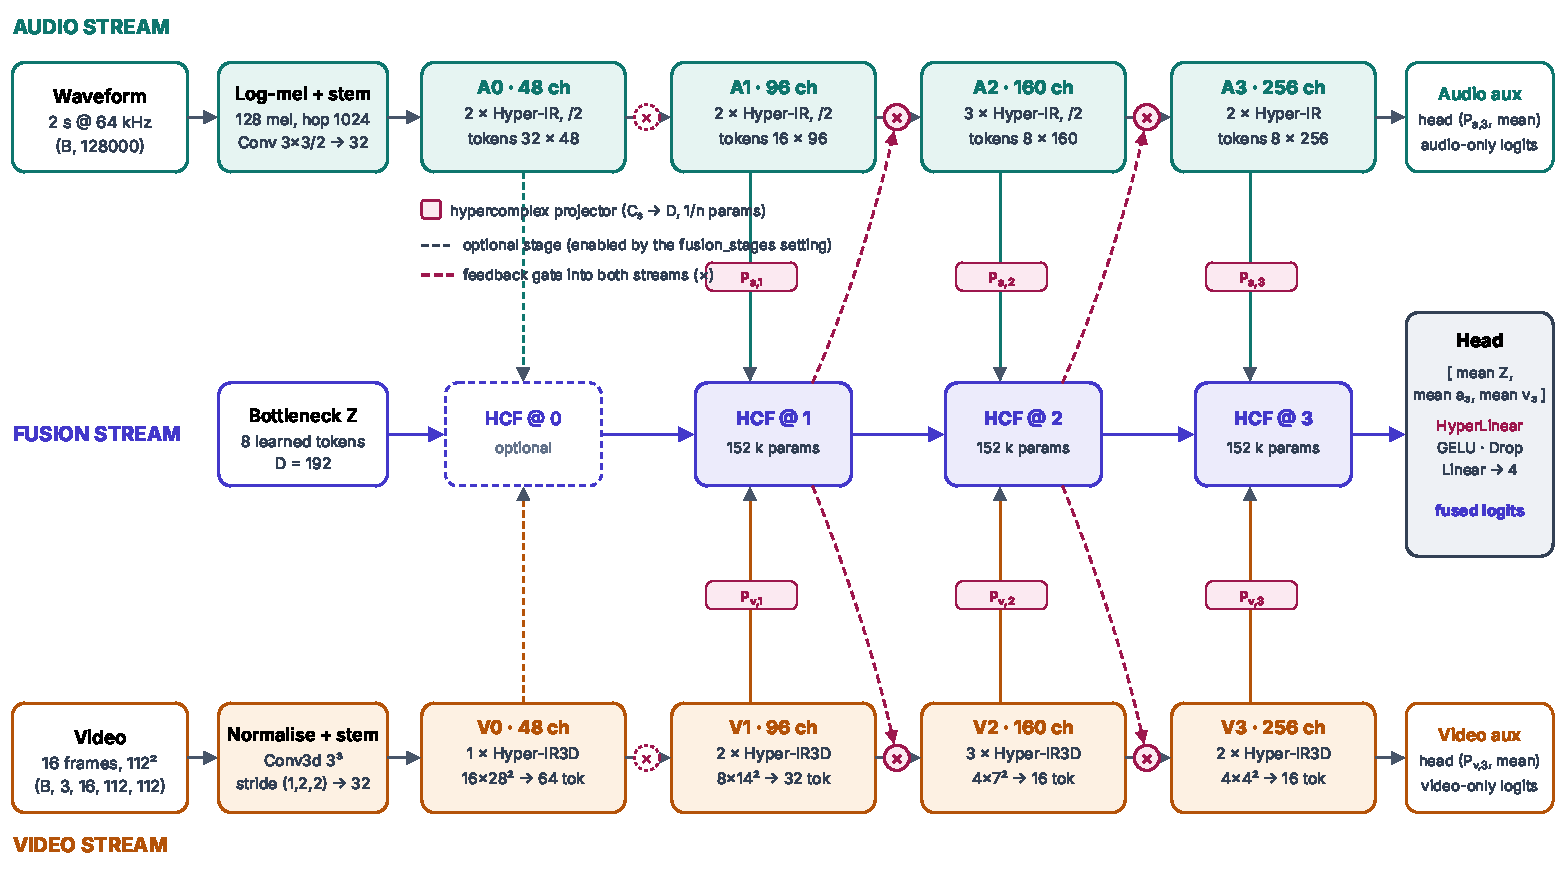
\includegraphics[width=\textwidth]{figures/arch_overview.pdf}
  \caption{HyperAVNet (default configuration: quaternion algebra, fusion stages $\mathcal{S}=\{1,2,3\}$,
  feedback enabled). Stage tokens of the audio and video backbones are projected by hypercomplex
  projectors $P_{a,s}$ and $P_{v,s}$ into a $D$-dimensional fusion space, where HCF blocks update the
  bottleneck tokens $\mathbf{Z}$. After each fused stage $s<S-1$, a zero-initialised gate ($\times$)
  modulates both streams. The classifier reads the pooled bottleneck and the pooled last-stage
  tokens; auxiliary heads supervise each modality on its own. Token shapes are for one 2\,s clip and
  $16\times112^{2}$ frames.}
  \label{fig:overview}
\end{figure*}

\subsection{Hypercomplex layers}
\label{sec:hyper}
Let $\mathbb{A}_n$ be a hypercomplex algebra of dimension $n\in\{2,4,8,16\}$ (complex numbers,
quaternions, octonions, sedenions, obtained by the Cayley--Dickson construction), with basis
$\{e_0,\dots,e_{n-1}\}$ and multiplication table
\begin{equation}
  e_i\,e_j = \sigma_{ij}\, e_{\pi(i,j)},
  \label{eq:table}
\end{equation}
with signs $\sigma_{ij}\in\{-1,+1\}$ and indices $\pi(i,j)\in\{0,\dots,n-1\}$.
A feature vector $\mathbf{x}\in\mathbb{R}^{d_{\mathrm{in}}}$ is split into $n$ components,
$\mathbf{x}=[\mathbf{x}_0;\dots;\mathbf{x}_{n-1}]$ with $\mathbf{x}_j\in\mathbb{R}^{d_{\mathrm{in}}/n}$,
i.e.\ it is read as $\sum_j \mathbf{x}_j e_j$. A hypercomplex weight
$\mathbf{W}=\sum_{k}\mathbf{W}_k e_k$ with real blocks $\mathbf{W}_k\in\mathbb{R}^{(d_{\mathrm{out}}/n)\times(d_{\mathrm{in}}/n)}$
acts on it by the algebra product, which in matrix form is
\begin{equation}
\begin{gathered}
  \mathbf{y}_i = \sum_{j=0}^{n-1} s_{ij}\,\mathbf{W}_{c(i,j)}\,\mathbf{x}_j + \mathbf{b}_i,\\
  \mathbf{K}(\mathbf{W}) = \big[\, s_{ij}\,\mathbf{W}_{c(i,j)} \,\big]_{i,j=0}^{n-1}\in\mathbb{R}^{d_{\mathrm{out}}\times d_{\mathrm{in}}},
\end{gathered}
  \label{eq:hlinear}
\end{equation}
where the block index $c(i,j)$ and sign $s_{ij}$ follow from Eq.~\eqref{eq:table}. For quaternions the
kernel takes the familiar Hamilton form (Fig.~\ref{fig:hamilton}),
\begin{equation}
  \mathbf{K} = \begin{bmatrix}
   \mathbf{W}_0 & \mathbf{W}_1 & \mathbf{W}_2 & \mathbf{W}_3\\
  -\mathbf{W}_1 & \mathbf{W}_0 & \mathbf{W}_3 & -\mathbf{W}_2\\
  -\mathbf{W}_2 & -\mathbf{W}_3 & \mathbf{W}_0 & \mathbf{W}_1\\
  -\mathbf{W}_3 & \mathbf{W}_2 & -\mathbf{W}_1 & \mathbf{W}_0
  \end{bmatrix}.
  \label{eq:hamilton}
\end{equation}
Every output component is thus a signed combination of \emph{every} input component through one
shared set of $n$ blocks, so the layer has
\begin{equation}
  |\theta_{\mathrm{hyper}}| = \tfrac{1}{n}\,d_{\mathrm{in}}d_{\mathrm{out}} + d_{\mathrm{out}}
  \;\;\text{vs.}\;\;
  |\theta_{\mathrm{real}}| = d_{\mathrm{in}}d_{\mathrm{out}} + d_{\mathrm{out}}
  \label{eq:params}
\end{equation}
parameters. A hypercomplex convolution applies the same block structure to the kernel tensor, with
$\mathbf{W}_k\in\mathbb{R}^{(C_{\mathrm{out}}/n)\times(C_{\mathrm{in}}/n)\times k_1\times\dots}$.
Weights are initialised in polar form: a modulus drawn from a $\chi$ distribution with $n$ degrees of
freedom (scaled by the Glorot variance), a uniform phase, and a unit-norm imaginary direction
\cite{bojesomo2024hypercomplex}. We write $\mathcal{H}_n(\cdot)$ for a hypercomplex linear or
convolutional layer. With $n=1$ it reduces to the real layer, which gives a matched real-valued
ablation with an identical code path.

\paragraph{Deployment.} Building $\mathbf{K}$ in Eq.~\eqref{eq:hlinear} at every forward pass
is only needed while training. After training, every $\mathcal{H}_n$ is \emph{reparameterised} into a
dense layer with weight $\mathbf{K}(\mathbf{W})$. The outputs are identical, and the run-time
overhead of kernel assembly disappears. The hypercomplex structure therefore reduces the number of
stored and optimised parameters (and the model's memory and transmission size) by up to $n\times$,
but \emph{not} the multiply--accumulate count, because $\mathbf{K}$ is dense.

\begin{figure}[t]
  \centering
  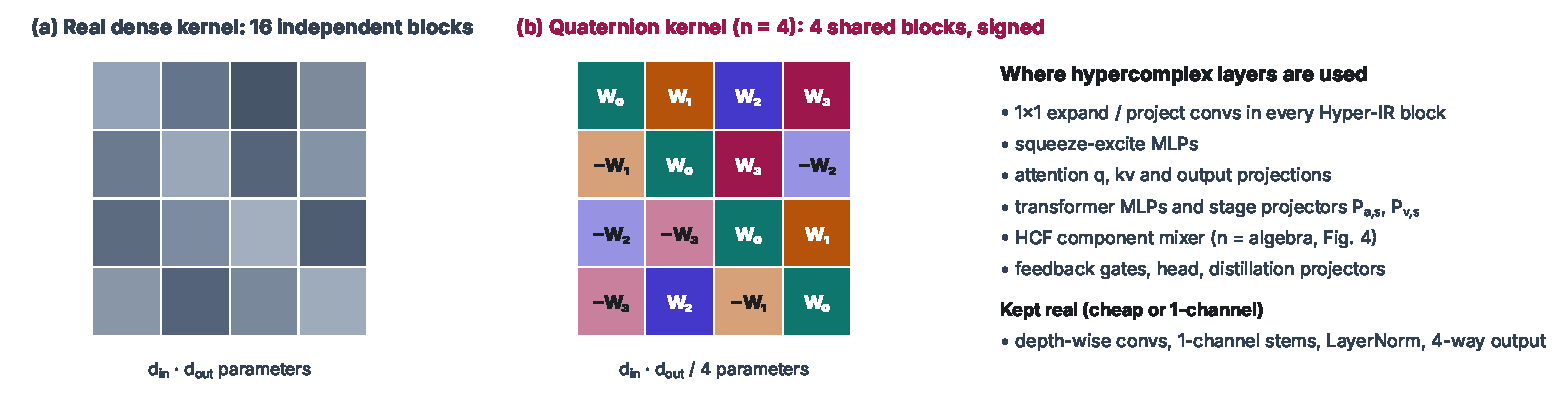
\includegraphics[width=\columnwidth]{figures/hamilton.pdf}
  \caption{Hamilton-product weight sharing. (a) A real kernel has $n^{2}$ independent blocks.
  (b) A quaternion kernel ($n=4$) re-uses four blocks with fixed signs (Eq.~\eqref{eq:hamilton}),
  which cuts the parameter count by $4\times$.}
  \label{fig:hamilton}
\end{figure}

\subsection{Hypercomplex backbones and stage tokens}
\label{sec:backbones}
\paragraph{Hyper-IR block.} Both backbones stack hypercomplex inverted-residual blocks
(Fig.~\ref{fig:hyperir}). For an input $\mathbf{h}\in\mathbb{R}^{C\times\Omega}$ ($\Omega$ is the 2-D
time--frequency grid for audio and the 3-D space--time grid for video) and expansion ratio $r=4$:
\begin{equation}
\begin{aligned}
  \mathbf{u} &= \operatorname{SiLU}\big(\operatorname{BN}(\mathcal{H}_n^{1\times1}(\mathbf{h}))\big)\in\mathbb{R}^{rC\times\Omega},\\
  \mathbf{v} &= \operatorname{SiLU}\big(\operatorname{BN}(\operatorname{DWConv}_{3}(\mathbf{u}))\big),\\
  \mathbf{w} &= \mathbf{v}\odot\sigma\big(\mathcal{H}_n(\operatorname{SiLU}(\mathcal{H}_n(\operatorname{GAP}(\mathbf{v}))))\big),\\
  \mathbf{h}' &= \mathbf{h} + \operatorname{DropPath}\big(\operatorname{BN}(\mathcal{H}_n^{1\times1}(\mathbf{w}))\big).
\end{aligned}
  \label{eq:hyperir}
\end{equation}
The two point-wise convolutions hold almost all of a block's parameters, so they are hypercomplex. The
depth-wise convolution stays real; it accounts for about 1\% of the parameters. The residual is used
when the shape is preserved.

\paragraph{Audio stream.} The waveform is converted to a log-mel spectrogram with the U-FFIA settings
(Hann window 2048, hop 1024, 128 mel bins at 64\,kHz, so a 2\,s clip gives $128\times126$),
normalised per mel bin by batch normalisation and augmented with SpecAugment during training. A
$3{\times}3$ stride-2 stem is followed by four Hyper-IR stages $s=0,\dots,3$ with widths
$(48,96,160,256)$ and depths $(2,2,3,2)$. A stage map $\mathbf{h}^{a}_{s}\in\mathbb{R}^{C_s\times T_s\times F_s}$
becomes time tokens by pooling over frequency:
\begin{equation}
  \mathbf{a}_s = \big[\operatorname{mean}_{F}(\mathbf{h}^{a}_s) + \operatorname{max}_{F}(\mathbf{h}^{a}_s)\big]^{\top}\in\mathbb{R}^{T_s\times C_s}.
  \label{eq:audiotokens}
\end{equation}
The max term keeps the short impulsive transients of feeding (chewing, tail slaps).

\paragraph{Video stream.} The frames are normalised and passed through a $3{\times}3{\times}3$ stem
(spatial stride 2) and four 3-D Hyper-IR stages of the same widths, with depths $(1,2,3,2)$ and
strides $(1,2,2)$, $(2,2,2)$, $(2,2,2)$, $(1,2,2)$. A stage map
$\mathbf{h}^{v}_{s}\in\mathbb{R}^{C_s\times T_s\times H_s\times W_s}$ is pooled to a $2\times2$ spatial grid
per time step, $\mathbf{v}_s\in\mathbb{R}^{4T_s\times C_s}$. This keeps coarse location (where the fish
aggregate) at a small token count.

\begin{figure}[t]
  \centering
  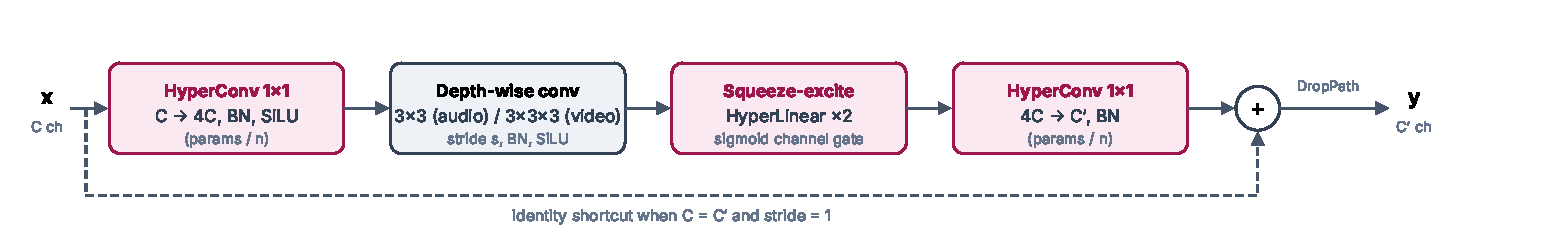
\includegraphics[width=\columnwidth]{figures/hyper_ir.pdf}
  \caption{Hypercomplex inverted-residual (Hyper-IR) block, Eq.~\eqref{eq:hyperir}. Hypercomplex
  layers are shaded; the depth-wise convolution is real.}
  \label{fig:hyperir}
\end{figure}

\paragraph{Pretrained backbones.} Any pretrained network can replace a student backbone if it exposes
four stages in the same token format. We use this for the teachers and for the teacher ablation
(Sec.~\ref{sec:setup}): PANNs CNN10/CNN14~\cite{kong2020panns}, EfficientAT~\cite{schmid2023efficientat},
AST~\cite{gong2021ast}, S3D~\cite{xie2018s3d}, X3D~\cite{feichtenhofer2020x3d},
MoViNet~\cite{kondratyuk2021movinets} and VideoMAE~\cite{tong2022videomae}. Their intermediate layers
supply the stage tokens.

\subsection{Hypercomplex component fusion}
\label{sec:hcf}
\paragraph{Projection.} Stage tokens are mapped into a shared $D$-dimensional space by hypercomplex
projectors with a learned modality embedding:
\begin{equation}
  \mathbf{A}_s = \operatorname{LN}\!\big(\mathcal{H}_n(\mathbf{a}_s)\big) + \mathbf{m}^{a},\qquad
  \mathbf{V}_s = \operatorname{LN}\!\big(\mathcal{H}_n(\mathbf{v}_s)\big) + \mathbf{m}^{v}.
  \label{eq:proj}
\end{equation}

\paragraph{Bottleneck state.} The fused representation lives in $N_b$ learned bottleneck tokens
$\mathbf{Z}\in\mathbb{R}^{N_b\times D}$ (we use $N_b=8$, $D=192$), shared across stages.

\paragraph{HCF block.} At a fusion stage $s$, the bottleneck first reads each modality with its own
hypercomplex cross-attention:
\begin{equation}
\begin{aligned}
  \mathbf{Z}^{a} &= \mathbf{Z} + \operatorname{XAttn}_{n}\big(\operatorname{LN}\mathbf{Z},\,\operatorname{LN}\mathbf{A}_s\big),\\
  \mathbf{Z}^{v} &= \mathbf{Z} + \operatorname{XAttn}_{n}\big(\operatorname{LN}\mathbf{Z},\,\operatorname{LN}\mathbf{V}_s\big),
\end{aligned}
  \label{eq:xattn}
\end{equation}
where $\operatorname{XAttn}_n$ is multi-head attention whose query, key, value and output projections
are hypercomplex (shown for one head of width $d_h$):
\begin{equation*}
  \operatorname{XAttn}_n(\mathbf{Q},\mathbf{C})=\mathcal{H}_n\Big(\operatorname{softmax}\Big(\tfrac{\mathcal{H}_n(\mathbf{Q})\,\mathcal{H}_n(\mathbf{C})^{\top}}{\sqrt{d_h}}\Big)\mathcal{H}_n(\mathbf{C})\Big).
\end{equation*} The shared
state, the two modality views and their interaction then form the components of one element of
$\mathbb{A}_m$:
\begin{equation}
  \mathbf{q} = \mathbf{Z}\,e_0 + \mathbf{Z}^{a}\,e_1 + \mathbf{Z}^{v}\,e_2 + \big(\hat{\mathbf{Z}}^{a}\odot\hat{\mathbf{Z}}^{v}\big)\,e_3,
  \label{eq:components}
\end{equation}
for $m=4$,
with $\hat{\cdot}=\operatorname{LN}(\cdot)$. The octonion variant ($m=8$) appends
$(\mathbf{Z}^{a}-\mathbf{Z}^{v})e_4$, $(\hat{\mathbf{Z}}\odot\hat{\mathbf{Z}}^{a})e_5$,
$(\hat{\mathbf{Z}}\odot\hat{\mathbf{Z}}^{v})e_6$ and
$(\hat{\mathbf{Z}}\odot\hat{\mathbf{Z}}^{a}\odot\hat{\mathbf{Z}}^{v})e_7$; the complex variant ($m=2$) uses
$(\mathbf{Z}^{a},\mathbf{Z}^{v})$. The components are mixed by a single Hamilton product, followed by a
hypercomplex MLP:
\begin{equation}
\begin{aligned}
  \mathbf{Z} &\leftarrow \mathbf{Z} + \boldsymbol{\gamma}_1\odot \mathcal{H}_m(\mathbf{q}),\\
  \mathbf{Z} &\leftarrow \mathbf{Z} + \boldsymbol{\gamma}_2\odot \operatorname{MLP}_n(\operatorname{LN}\mathbf{Z}),
\end{aligned}
  \label{eq:mix}
\end{equation}
where $\mathcal{H}_m:\mathbb{R}^{mD}\to\mathbb{R}^{D}$ is a hypercomplex linear layer of algebra
$\mathbb{A}_m$ and $\boldsymbol{\gamma}_{1,2}$ are LayerScale vectors~\cite{touvron2021cait}, initialised to
$10^{-2}$. By Eq.~\eqref{eq:hlinear}, each output component of $\mathcal{H}_m$ is a signed mixture of
the shared state, both modality views and their multiplicative agreement, all through one set of
$m$ blocks. The mixer has $D^{2}$ parameters \emph{for every} $m$, against $mD^{2}$ for a dense mixer, so
the octonion variant adds four interaction terms at no parameter cost. Unlike attention bottlenecks
that attend to the modalities one after the other~\cite{nagrani2021mbt}, HCF reads both modalities
in parallel and combines them in one algebraic product (Fig.~\ref{fig:hcf}).

\begin{figure*}[t]
  \centering
  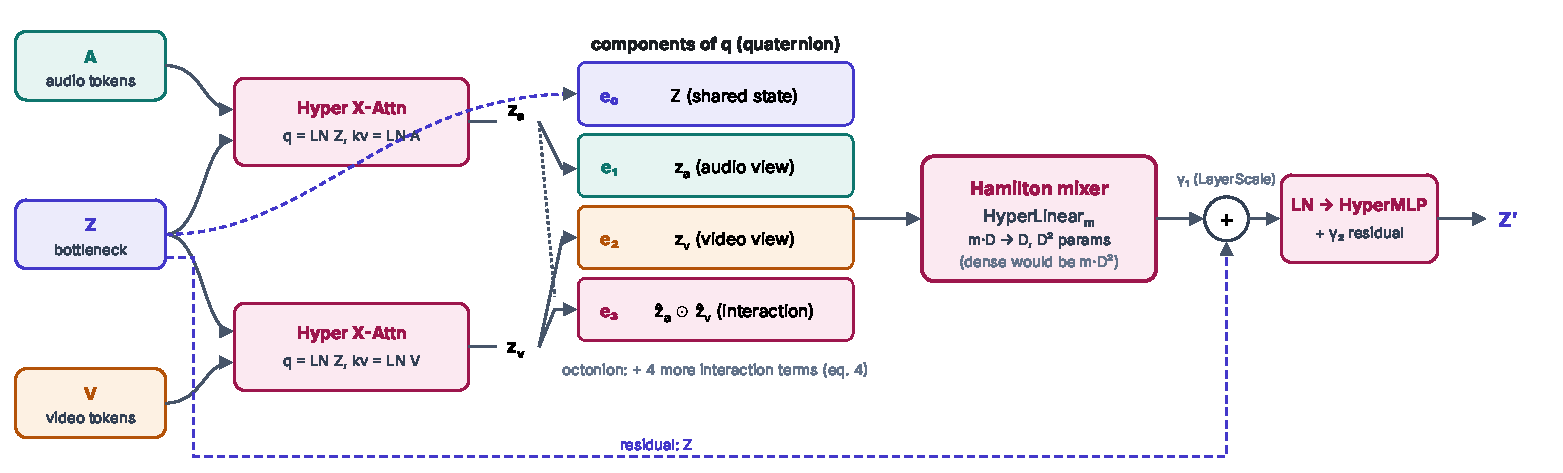
\includegraphics[width=0.9\textwidth]{figures/hcf_block.pdf}
  \caption{Hypercomplex component fusion (HCF), Eqs.~\eqref{eq:xattn}--\eqref{eq:mix}. The modality
  views and their interaction are the components of one quaternion and are mixed by a single
  Hamilton product.}
  \label{fig:hcf}
\end{figure*}

\subsection{Deep-to-early fusion schedule with cross-modal feedback}
\label{sec:schedule}
The set $\mathcal{S}\subseteq\{0,\dots,S-1\}$ selects the stages at which an HCF block is attached:
\begin{equation}
  \mathbf{Z}^{(s+1)} = \begin{cases}\operatorname{HCF}_s\big(\mathbf{Z}^{(s)},\mathbf{A}_s,\mathbf{V}_s\big), & s\in\mathcal{S},\\ \mathbf{Z}^{(s)}, & \text{otherwise,}\end{cases}
  \label{eq:schedule}
\end{equation}
with $\mathbf{Z}^{(0)}=\mathbf{Z}_{\mathrm{init}}$ the learned bottleneck tokens.
Varying $\mathcal{S}$ from $\{S-1\}$ (late fusion) through $\{S-2,S-1\}$ and so on to $\{0,\dots,S-1\}$
gives a controlled \emph{deep-to-early} study of where audio--visual fusion helps. Because the student
backbones are executed stage by stage, the fused state is also fed back into both streams after each
fused stage $s<S-1$:
\begin{equation}
  \mathbf{h}^{m}_s \leftarrow \mathbf{h}^{m}_s\odot\big(1+\tanh(\mathcal{G}^{m}_s\,\bar{\mathbf{z}}^{(s+1)})\big),\quad m\in\{a,v\},
  \label{eq:feedback}
\end{equation}
where $\bar{\mathbf{z}}=\operatorname{mean}_{N_b}(\mathbf{Z})$, the gates
$\mathcal{G}^{m}_s$ are hypercomplex linear maps $\mathbb{R}^{D}\to\mathbb{R}^{C_s}$, and the
product broadcasts over $\Omega$. The gates are \emph{initialised to zero}, so training starts exactly
at the feedback-free model. The network then learns how strongly each modality should condition the
other's later features. This is genuine early fusion, as opposed to fusing independently computed
features.

\subsection{Prediction heads and modality dropout}
\label{sec:heads}
With $\bar{\mathbf{z}}=\operatorname{mean}(\operatorname{LN}\mathbf{Z}^{(S)})$,
$\bar{\mathbf{a}}=\operatorname{mean}(\operatorname{LN}\mathbf{A}_{S-1})$ and
$\bar{\mathbf{v}}=\operatorname{mean}(\operatorname{LN}\mathbf{V}_{S-1})$, the fused and auxiliary logits are
\begin{equation}
\begin{gathered}
  \boldsymbol{\ell} = \mathbf{W}_o\,\operatorname{GELU}\big(\mathcal{H}_n[\bar{\mathbf{z}};\,\mu_a\bar{\mathbf{a}};\,\mu_v\bar{\mathbf{v}}]\big),\\
  \boldsymbol{\ell}^{a} = \mathbf{W}_a\bar{\mathbf{a}},\qquad \boldsymbol{\ell}^{v} = \mathbf{W}_v\bar{\mathbf{v}}.
\end{gathered}
  \label{eq:heads}
\end{equation}
Here $\mu_a,\mu_v\in\{0,1\}$ are per-sample modality masks. During training,
$(\mu_a,\mu_v)=(0,1)$ with probability $p$, $(1,0)$ with probability $p$, and $(1,1)$ otherwise. In the
notation of~\cite{cui2024uffia}, $p_{av}=1-2p$ and $p_a=p_v=p$. The same mask multiplies every fusion
input $\mathbf{A}_s,\mathbf{V}_s$, so a dropped modality is absent everywhere. The auxiliary heads always see
their own modality, which keeps both branches trained regardless of $p$. At test time, forcing
$\mu_a=0$ or $\mu_v=0$ evaluates the model with a missing modality.

\subsection{Training objective and multi-level distillation}
\label{sec:objective}
The supervised loss combines label-smoothed cross-entropy on the fused logits with the two
auxiliary terms:
\begin{equation}
  \mathcal{L}_{\mathrm{sup}} = \operatorname{CE}_{\epsilon}(\boldsymbol{\ell},y)
   + \tfrac{\lambda_{\mathrm{aux}}}{2}\!\!\sum_{m\in\{a,v\}}\!\!\operatorname{CE}_{\epsilon}(\boldsymbol{\ell}^{m},y).
  \label{eq:sup}
\end{equation}
A frozen teacher $g$ with the same output structure (pretrained backbones and HCF fusion) provides
three further signals. At the \emph{logit level}, with temperature $\tau$:
\begin{equation}
  \mathcal{L}_{\mathrm{KD}} = \tau^{2}\,\mathrm{KL}\big(\boldsymbol{\ell}^{g}\,\|\,\boldsymbol{\ell}\big)_{\tau}
   + \tfrac{\lambda_{u}\tau^{2}}{2}\!\!\sum_{m\in\{a,v\}}\!\!\mathrm{KL}\big(\boldsymbol{\ell}^{g,m}\,\|\,\boldsymbol{\ell}^{m}\big)_{\tau},
  \label{eq:kd}
\end{equation}
with $\mathrm{KL}(\mathbf{u}\,\|\,\mathbf{w})_{\tau}=\mathrm{KL}\big(\operatorname{softmax}(\mathbf{u}/\tau)\,\|\,\operatorname{softmax}(\mathbf{w}/\tau)\big)$,
which distils each unimodal head from its counterpart in the teacher. U-FFIA's variant~\cite{cui2024uffia}
softens only the teacher, $\mathrm{KL}(\operatorname{softmax}(\boldsymbol{\ell}^{g}/\tau)\,\|\,\operatorname{softmax}(\boldsymbol{\ell}))$,
and is evaluated as an ablation. At the \emph{embedding level}, small hypercomplex projectors
$\mathcal{P}_k$ align the student's pooled embeddings with the teacher's:
\begin{equation}
  \mathcal{L}_{\mathrm{feat}} = \tfrac{1}{3}\!\!\sum_{k\in\{\bar{\mathbf{z}},\bar{\mathbf{a}},\bar{\mathbf{v}}\}}\!\!
  \big(1-\cos(\mathcal{P}_k(k),\,k^{g})\big).
  \label{eq:feat}
\end{equation}
At the \emph{relation level}~\cite{park2019rkd}, the within-batch similarity structure of the fused
embeddings is matched:
\begin{equation}
  \mathcal{L}_{\mathrm{rel}} = \operatorname{SmoothL1}\big(\mathbf{R}(\bar{\mathbf{z}}_{1:B}),\,\mathbf{R}(\bar{\mathbf{z}}^{g}_{1:B})\big),
  \label{eq:rel}
\end{equation}
where $\mathbf{R}(\mathbf{U})_{ij}=\mathbf{u}_i^{\top}\mathbf{u}_j/(\|\mathbf{u}_i\|\|\mathbf{u}_j\|)$ is the cosine-similarity matrix of a batch of size $B$.
The full objective is
\begin{equation}
  \mathcal{L} = \mathcal{L}_{\mathrm{sup}} + \alpha\,\mathcal{L}_{\mathrm{KD}} + \beta\,\mathcal{L}_{\mathrm{feat}} + \gamma\,\mathcal{L}_{\mathrm{rel}},
  \label{eq:total}
\end{equation}
with $\epsilon=0.1$, $\lambda_{\mathrm{aux}}=0.3$, $\lambda_u=0.5$, $\tau=2$, $\alpha=0.7$, $\beta=1$ and $\gamma=0.5$.
Training proceeds in two stages: the teacher is trained with $\mathcal{L}_{\mathrm{sup}}$ and frozen, then
the student is trained with Eq.~\eqref{eq:total}.

\begin{figure*}[t]
  \centering
  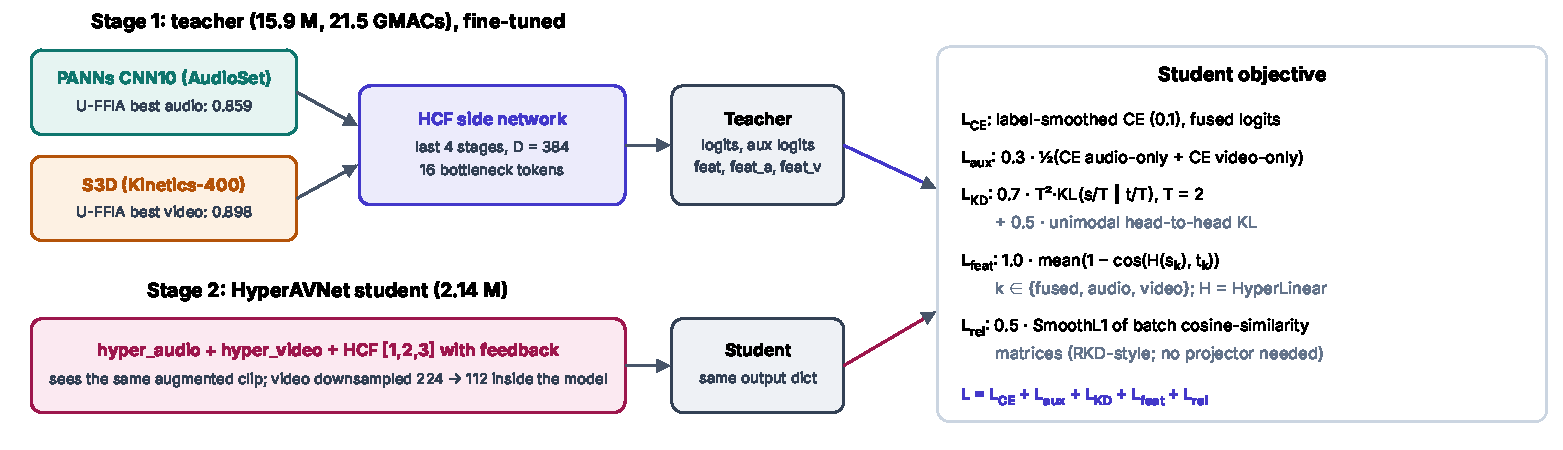
\includegraphics[width=0.92\textwidth]{figures/distillation.pdf}
  \caption{Two-stage training. A teacher built from pretrained audio and video backbones and HCF fusion
  is trained first and frozen. The HyperAVNet student is then trained with the supervised loss plus
  logit-, embedding- and relation-level distillation (Eq.~\eqref{eq:total}).}
  \label{fig:distill}
\end{figure*}

\subsection{Complexity}
\label{sec:complexity}
By Eq.~\eqref{eq:params}, every hypercomplex projection stores $1/n$ of the real parameters. Only the
stems, the depth-wise convolutions, normalisation layers and the final $4$-way classifier stay real.
For the default student ($n=4$), the network has 2.14\,M parameters against 7.88\,M for the identical
real network ($n=1$), and 1.24\,M (octonion) or 0.78\,M (sedenion) for higher algebras. Compute is
1.18\,GMACs per clip for every $n$ (16 frames at $112^{2}$ and 2\,s of audio). The added cost of a
fusion stage is about 0.17\,M parameters and under 0.02\,GMACs.
 in any paper.
%  Requires: amsmath, amssymb, bm, booktabs, graphicx, (cleveref optional).
% ============================================================================
\section{Methodology}
\label{sec:method}

\subsection{Problem formulation}
\label{sec:problem}
Each sample of AV-FFIA is a synchronised two-second clip $(\mathbf{x}^{a}, \mathbf{X}^{v})$, where
$\mathbf{x}^{a}\in\mathbb{R}^{L}$ is the hydrophone waveform ($L = 2f_s$, $f_s = 64$\,kHz) and
$\mathbf{X}^{v}\in[0,1]^{3\times T\times H\times W}$ holds $T$ RGB frames sampled uniformly from the
overhead camera. The label $y\in\mathcal{Y}=\{\textsc{None},\textsc{Weak},\textsc{Medium},\textsc{Strong}\}$
is the feeding intensity. We learn $f_{\theta}:(\mathbf{x}^{a},\mathbf{X}^{v})\mapsto\mathbf{p}\in\Delta^{|\mathcal{Y}|-1}$ with
two goals that pull in opposite directions: high accuracy, robust to the acoustic and visual
corruptions typical of aquaculture (bubbles, pumps, low light, reflections), and a small
parameter and compute budget for on-site deployment.

HyperAVNet (Fig.~\ref{fig:overview}) has four parts. Two hypercomplex backbones map each modality to a
hierarchy of \emph{stage tokens} (Sec.~\ref{sec:backbones}). A set of shared \emph{bottleneck tokens}
is updated by hypercomplex component fusion (HCF) blocks attached at a configurable subset of
stages, with zero-initialised cross-modal feedback into both streams (Secs.~\ref{sec:hcf},~\ref{sec:schedule}).
Fused and unimodal heads produce the predictions (Sec.~\ref{sec:heads}). The model is trained with a
multi-level distillation objective from a pretrained audio-visual teacher (Sec.~\ref{sec:objective}).

\begin{figure*}[t]
  \centering
  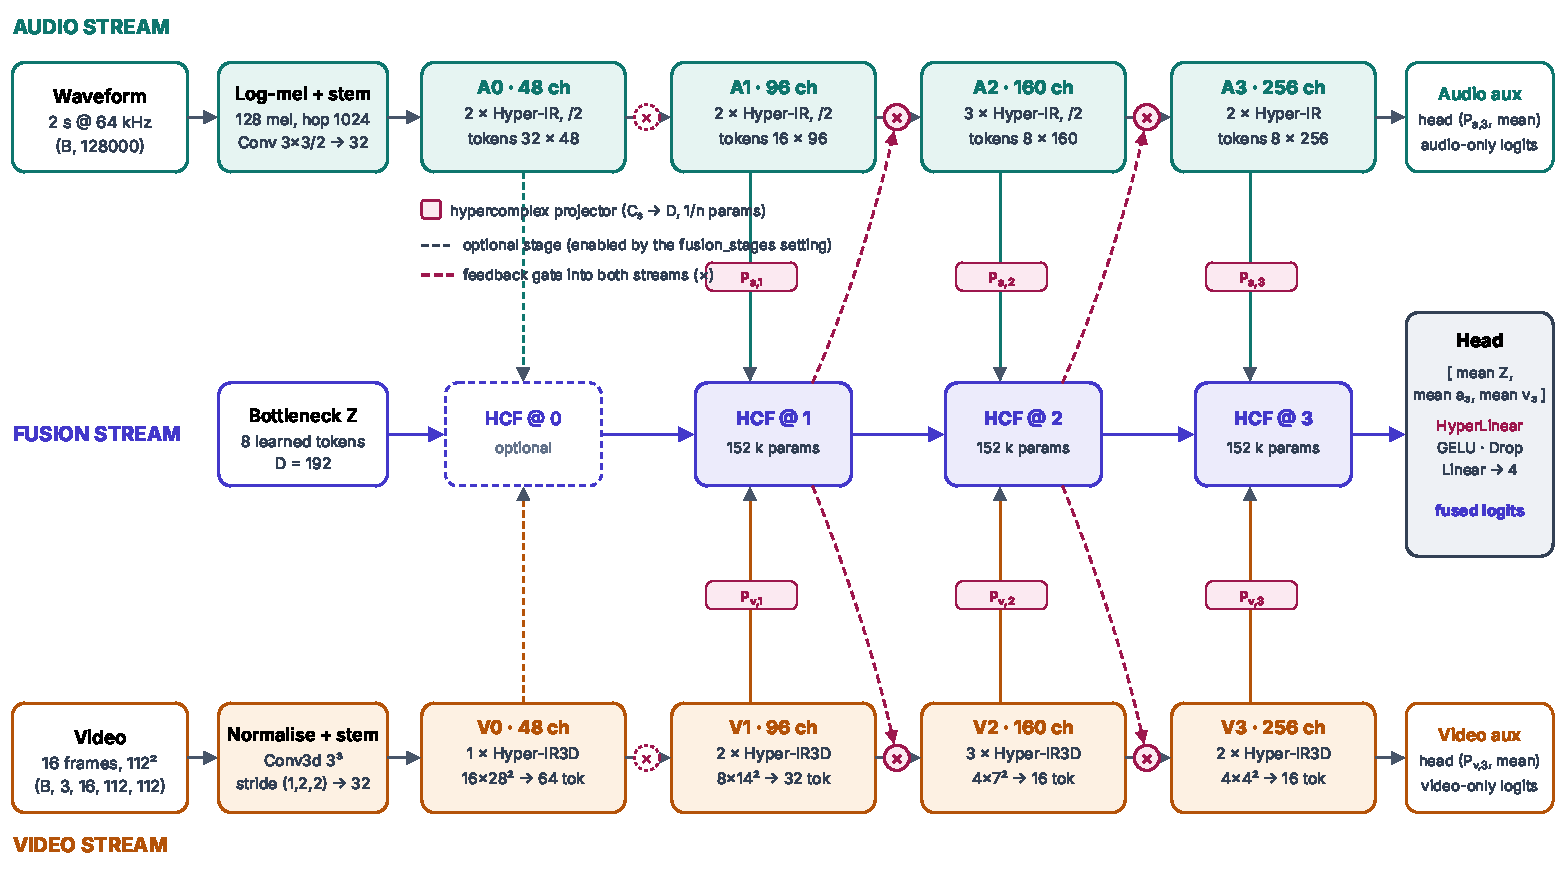
\includegraphics[width=\textwidth]{figures/arch_overview.pdf}
  \caption{HyperAVNet (default configuration: quaternion algebra, fusion stages $\mathcal{S}=\{1,2,3\}$,
  feedback enabled). Stage tokens of the audio and video backbones are projected by hypercomplex
  projectors $P_{a,s}$ and $P_{v,s}$ into a $D$-dimensional fusion space, where HCF blocks update the
  bottleneck tokens $\mathbf{Z}$. After each fused stage $s<S-1$, a zero-initialised gate ($\times$)
  modulates both streams. The classifier reads the pooled bottleneck and the pooled last-stage
  tokens; auxiliary heads supervise each modality on its own. Token shapes are for one 2\,s clip and
  $16\times112^{2}$ frames.}
  \label{fig:overview}
\end{figure*}

\subsection{Hypercomplex layers}
\label{sec:hyper}
Let $\mathbb{A}_n$ be a hypercomplex algebra of dimension $n\in\{2,4,8,16\}$ (complex numbers,
quaternions, octonions, sedenions, obtained by the Cayley--Dickson construction), with basis
$\{e_0,\dots,e_{n-1}\}$ and multiplication table
\begin{equation}
  e_i\,e_j = \sigma_{ij}\, e_{\pi(i,j)},
  \label{eq:table}
\end{equation}
with signs $\sigma_{ij}\in\{-1,+1\}$ and indices $\pi(i,j)\in\{0,\dots,n-1\}$.
A feature vector $\mathbf{x}\in\mathbb{R}^{d_{\mathrm{in}}}$ is split into $n$ components,
$\mathbf{x}=[\mathbf{x}_0;\dots;\mathbf{x}_{n-1}]$ with $\mathbf{x}_j\in\mathbb{R}^{d_{\mathrm{in}}/n}$,
i.e.\ it is read as $\sum_j \mathbf{x}_j e_j$. A hypercomplex weight
$\mathbf{W}=\sum_{k}\mathbf{W}_k e_k$ with real blocks $\mathbf{W}_k\in\mathbb{R}^{(d_{\mathrm{out}}/n)\times(d_{\mathrm{in}}/n)}$
acts on it by the algebra product, which in matrix form is
\begin{equation}
\begin{gathered}
  \mathbf{y}_i = \sum_{j=0}^{n-1} s_{ij}\,\mathbf{W}_{c(i,j)}\,\mathbf{x}_j + \mathbf{b}_i,\\
  \mathbf{K}(\mathbf{W}) = \big[\, s_{ij}\,\mathbf{W}_{c(i,j)} \,\big]_{i,j=0}^{n-1}\in\mathbb{R}^{d_{\mathrm{out}}\times d_{\mathrm{in}}},
\end{gathered}
  \label{eq:hlinear}
\end{equation}
where the block index $c(i,j)$ and sign $s_{ij}$ follow from Eq.~\eqref{eq:table}. For quaternions the
kernel takes the familiar Hamilton form (Fig.~\ref{fig:hamilton}),
\begin{equation}
  \mathbf{K} = \begin{bmatrix}
   \mathbf{W}_0 & \mathbf{W}_1 & \mathbf{W}_2 & \mathbf{W}_3\\
  -\mathbf{W}_1 & \mathbf{W}_0 & \mathbf{W}_3 & -\mathbf{W}_2\\
  -\mathbf{W}_2 & -\mathbf{W}_3 & \mathbf{W}_0 & \mathbf{W}_1\\
  -\mathbf{W}_3 & \mathbf{W}_2 & -\mathbf{W}_1 & \mathbf{W}_0
  \end{bmatrix}.
  \label{eq:hamilton}
\end{equation}
Every output component is thus a signed combination of \emph{every} input component through one
shared set of $n$ blocks, so the layer has
\begin{equation}
  |\theta_{\mathrm{hyper}}| = \tfrac{1}{n}\,d_{\mathrm{in}}d_{\mathrm{out}} + d_{\mathrm{out}}
  \;\;\text{vs.}\;\;
  |\theta_{\mathrm{real}}| = d_{\mathrm{in}}d_{\mathrm{out}} + d_{\mathrm{out}}
  \label{eq:params}
\end{equation}
parameters. A hypercomplex convolution applies the same block structure to the kernel tensor, with
$\mathbf{W}_k\in\mathbb{R}^{(C_{\mathrm{out}}/n)\times(C_{\mathrm{in}}/n)\times k_1\times\dots}$.
Weights are initialised in polar form: a modulus drawn from a $\chi$ distribution with $n$ degrees of
freedom (scaled by the Glorot variance), a uniform phase, and a unit-norm imaginary direction
\cite{bojesomo2024hypercomplex}. We write $\mathcal{H}_n(\cdot)$ for a hypercomplex linear or
convolutional layer. With $n=1$ it reduces to the real layer, which gives a matched real-valued
ablation with an identical code path.

\paragraph{Deployment.} Building $\mathbf{K}$ in Eq.~\eqref{eq:hlinear} at every forward pass
is only needed while training. After training, every $\mathcal{H}_n$ is \emph{reparameterised} into a
dense layer with weight $\mathbf{K}(\mathbf{W})$. The outputs are identical, and the run-time
overhead of kernel assembly disappears. The hypercomplex structure therefore reduces the number of
stored and optimised parameters (and the model's memory and transmission size) by up to $n\times$,
but \emph{not} the multiply--accumulate count, because $\mathbf{K}$ is dense.

\begin{figure}[t]
  \centering
  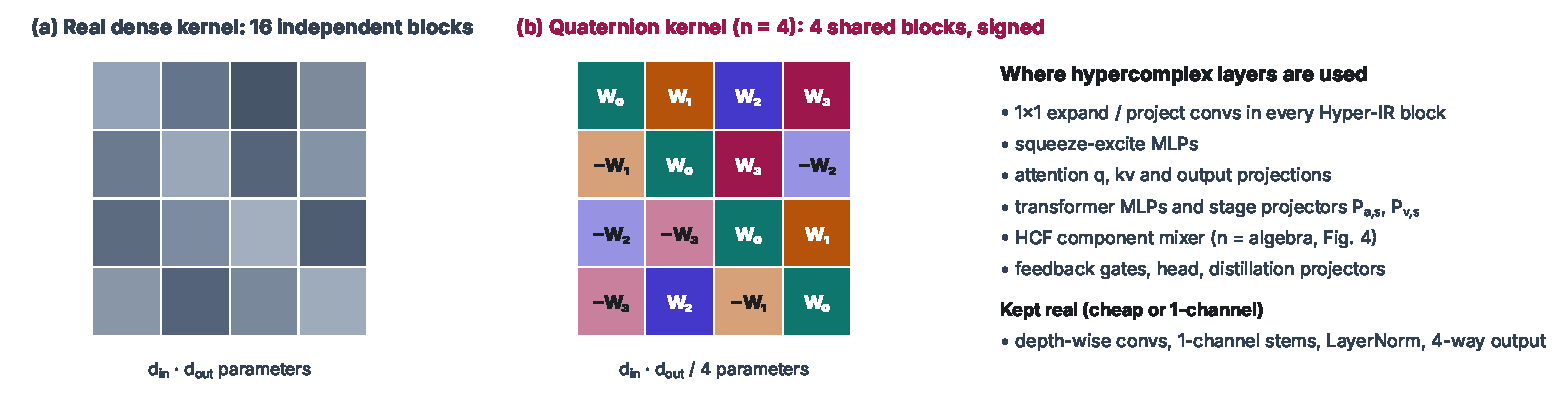
\includegraphics[width=\columnwidth]{figures/hamilton.pdf}
  \caption{Hamilton-product weight sharing. (a) A real kernel has $n^{2}$ independent blocks.
  (b) A quaternion kernel ($n=4$) re-uses four blocks with fixed signs (Eq.~\eqref{eq:hamilton}),
  which cuts the parameter count by $4\times$.}
  \label{fig:hamilton}
\end{figure}

\subsection{Hypercomplex backbones and stage tokens}
\label{sec:backbones}
\paragraph{Hyper-IR block.} Both backbones stack hypercomplex inverted-residual blocks
(Fig.~\ref{fig:hyperir}). For an input $\mathbf{h}\in\mathbb{R}^{C\times\Omega}$ ($\Omega$ is the 2-D
time--frequency grid for audio and the 3-D space--time grid for video) and expansion ratio $r=4$:
\begin{equation}
\begin{aligned}
  \mathbf{u} &= \operatorname{SiLU}\big(\operatorname{BN}(\mathcal{H}_n^{1\times1}(\mathbf{h}))\big)\in\mathbb{R}^{rC\times\Omega},\\
  \mathbf{v} &= \operatorname{SiLU}\big(\operatorname{BN}(\operatorname{DWConv}_{3}(\mathbf{u}))\big),\\
  \mathbf{w} &= \mathbf{v}\odot\sigma\big(\mathcal{H}_n(\operatorname{SiLU}(\mathcal{H}_n(\operatorname{GAP}(\mathbf{v}))))\big),\\
  \mathbf{h}' &= \mathbf{h} + \operatorname{DropPath}\big(\operatorname{BN}(\mathcal{H}_n^{1\times1}(\mathbf{w}))\big).
\end{aligned}
  \label{eq:hyperir}
\end{equation}
The two point-wise convolutions hold almost all of a block's parameters, so they are hypercomplex. The
depth-wise convolution stays real; it accounts for about 1\% of the parameters. The residual is used
when the shape is preserved.

\paragraph{Audio stream.} The waveform is converted to a log-mel spectrogram with the U-FFIA settings
(Hann window 2048, hop 1024, 128 mel bins at 64\,kHz, so a 2\,s clip gives $128\times126$),
normalised per mel bin by batch normalisation and augmented with SpecAugment during training. A
$3{\times}3$ stride-2 stem is followed by four Hyper-IR stages $s=0,\dots,3$ with widths
$(48,96,160,256)$ and depths $(2,2,3,2)$. A stage map $\mathbf{h}^{a}_{s}\in\mathbb{R}^{C_s\times T_s\times F_s}$
becomes time tokens by pooling over frequency:
\begin{equation}
  \mathbf{a}_s = \big[\operatorname{mean}_{F}(\mathbf{h}^{a}_s) + \operatorname{max}_{F}(\mathbf{h}^{a}_s)\big]^{\top}\in\mathbb{R}^{T_s\times C_s}.
  \label{eq:audiotokens}
\end{equation}
The max term keeps the short impulsive transients of feeding (chewing, tail slaps).

\paragraph{Video stream.} The frames are normalised and passed through a $3{\times}3{\times}3$ stem
(spatial stride 2) and four 3-D Hyper-IR stages of the same widths, with depths $(1,2,3,2)$ and
strides $(1,2,2)$, $(2,2,2)$, $(2,2,2)$, $(1,2,2)$. A stage map
$\mathbf{h}^{v}_{s}\in\mathbb{R}^{C_s\times T_s\times H_s\times W_s}$ is pooled to a $2\times2$ spatial grid
per time step, $\mathbf{v}_s\in\mathbb{R}^{4T_s\times C_s}$. This keeps coarse location (where the fish
aggregate) at a small token count.

\begin{figure}[t]
  \centering
  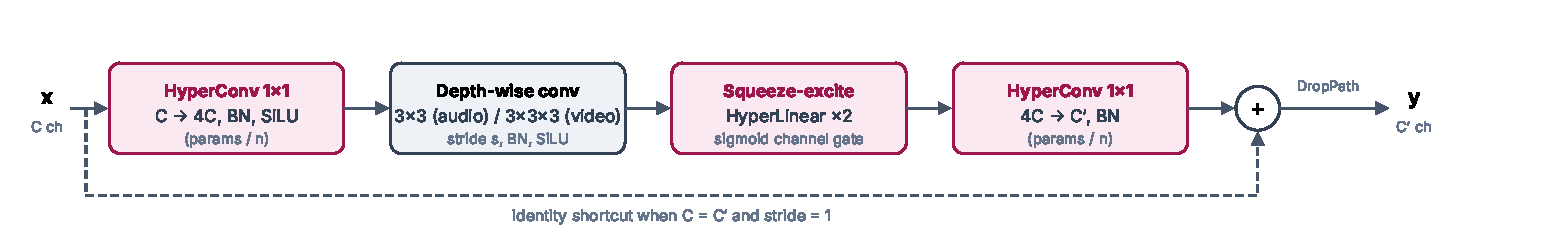
\includegraphics[width=\columnwidth]{figures/hyper_ir.pdf}
  \caption{Hypercomplex inverted-residual (Hyper-IR) block, Eq.~\eqref{eq:hyperir}. Hypercomplex
  layers are shaded; the depth-wise convolution is real.}
  \label{fig:hyperir}
\end{figure}

\paragraph{Pretrained backbones.} Any pretrained network can replace a student backbone if it exposes
four stages in the same token format. We use this for the teachers and for the teacher ablation
(Sec.~\ref{sec:setup}): PANNs CNN10/CNN14~\cite{kong2020panns}, EfficientAT~\cite{schmid2023efficientat},
AST~\cite{gong2021ast}, S3D~\cite{xie2018s3d}, X3D~\cite{feichtenhofer2020x3d},
MoViNet~\cite{kondratyuk2021movinets} and VideoMAE~\cite{tong2022videomae}. Their intermediate layers
supply the stage tokens.

\subsection{Hypercomplex component fusion}
\label{sec:hcf}
\paragraph{Projection.} Stage tokens are mapped into a shared $D$-dimensional space by hypercomplex
projectors with a learned modality embedding:
\begin{equation}
  \mathbf{A}_s = \operatorname{LN}\!\big(\mathcal{H}_n(\mathbf{a}_s)\big) + \mathbf{m}^{a},\qquad
  \mathbf{V}_s = \operatorname{LN}\!\big(\mathcal{H}_n(\mathbf{v}_s)\big) + \mathbf{m}^{v}.
  \label{eq:proj}
\end{equation}

\paragraph{Bottleneck state.} The fused representation lives in $N_b$ learned bottleneck tokens
$\mathbf{Z}\in\mathbb{R}^{N_b\times D}$ (we use $N_b=8$, $D=192$), shared across stages.

\paragraph{HCF block.} At a fusion stage $s$, the bottleneck first reads each modality with its own
hypercomplex cross-attention:
\begin{equation}
\begin{aligned}
  \mathbf{Z}^{a} &= \mathbf{Z} + \operatorname{XAttn}_{n}\big(\operatorname{LN}\mathbf{Z},\,\operatorname{LN}\mathbf{A}_s\big),\\
  \mathbf{Z}^{v} &= \mathbf{Z} + \operatorname{XAttn}_{n}\big(\operatorname{LN}\mathbf{Z},\,\operatorname{LN}\mathbf{V}_s\big),
\end{aligned}
  \label{eq:xattn}
\end{equation}
where $\operatorname{XAttn}_n$ is multi-head attention whose query, key, value and output projections
are hypercomplex (shown for one head of width $d_h$):
\begin{equation*}
  \operatorname{XAttn}_n(\mathbf{Q},\mathbf{C})=\mathcal{H}_n\Big(\operatorname{softmax}\Big(\tfrac{\mathcal{H}_n(\mathbf{Q})\,\mathcal{H}_n(\mathbf{C})^{\top}}{\sqrt{d_h}}\Big)\mathcal{H}_n(\mathbf{C})\Big).
\end{equation*} The shared
state, the two modality views and their interaction then form the components of one element of
$\mathbb{A}_m$:
\begin{equation}
  \mathbf{q} = \mathbf{Z}\,e_0 + \mathbf{Z}^{a}\,e_1 + \mathbf{Z}^{v}\,e_2 + \big(\hat{\mathbf{Z}}^{a}\odot\hat{\mathbf{Z}}^{v}\big)\,e_3,
  \label{eq:components}
\end{equation}
for $m=4$,
with $\hat{\cdot}=\operatorname{LN}(\cdot)$. The octonion variant ($m=8$) appends
$(\mathbf{Z}^{a}-\mathbf{Z}^{v})e_4$, $(\hat{\mathbf{Z}}\odot\hat{\mathbf{Z}}^{a})e_5$,
$(\hat{\mathbf{Z}}\odot\hat{\mathbf{Z}}^{v})e_6$ and
$(\hat{\mathbf{Z}}\odot\hat{\mathbf{Z}}^{a}\odot\hat{\mathbf{Z}}^{v})e_7$; the complex variant ($m=2$) uses
$(\mathbf{Z}^{a},\mathbf{Z}^{v})$. The components are mixed by a single Hamilton product, followed by a
hypercomplex MLP:
\begin{equation}
\begin{aligned}
  \mathbf{Z} &\leftarrow \mathbf{Z} + \boldsymbol{\gamma}_1\odot \mathcal{H}_m(\mathbf{q}),\\
  \mathbf{Z} &\leftarrow \mathbf{Z} + \boldsymbol{\gamma}_2\odot \operatorname{MLP}_n(\operatorname{LN}\mathbf{Z}),
\end{aligned}
  \label{eq:mix}
\end{equation}
where $\mathcal{H}_m:\mathbb{R}^{mD}\to\mathbb{R}^{D}$ is a hypercomplex linear layer of algebra
$\mathbb{A}_m$ and $\boldsymbol{\gamma}_{1,2}$ are LayerScale vectors~\cite{touvron2021cait}, initialised to
$10^{-2}$. By Eq.~\eqref{eq:hlinear}, each output component of $\mathcal{H}_m$ is a signed mixture of
the shared state, both modality views and their multiplicative agreement, all through one set of
$m$ blocks. The mixer has $D^{2}$ parameters \emph{for every} $m$, against $mD^{2}$ for a dense mixer, so
the octonion variant adds four interaction terms at no parameter cost. Unlike attention bottlenecks
that attend to the modalities one after the other~\cite{nagrani2021mbt}, HCF reads both modalities
in parallel and combines them in one algebraic product (Fig.~\ref{fig:hcf}).

\begin{figure*}[t]
  \centering
  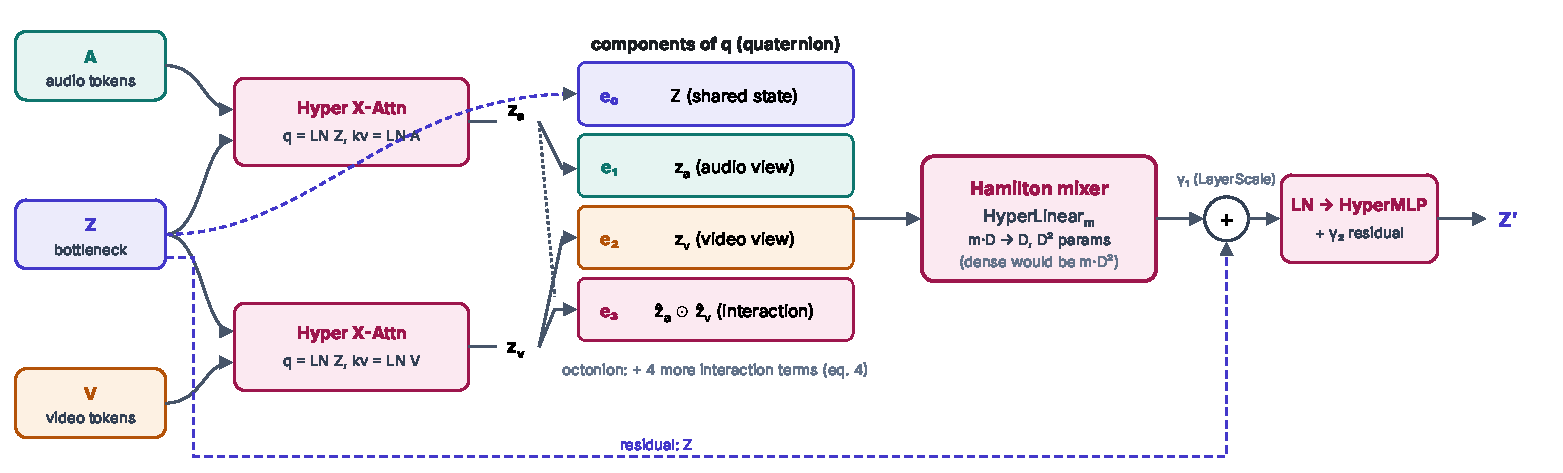
\includegraphics[width=0.9\textwidth]{figures/hcf_block.pdf}
  \caption{Hypercomplex component fusion (HCF), Eqs.~\eqref{eq:xattn}--\eqref{eq:mix}. The modality
  views and their interaction are the components of one quaternion and are mixed by a single
  Hamilton product.}
  \label{fig:hcf}
\end{figure*}

\subsection{Deep-to-early fusion schedule with cross-modal feedback}
\label{sec:schedule}
The set $\mathcal{S}\subseteq\{0,\dots,S-1\}$ selects the stages at which an HCF block is attached:
\begin{equation}
  \mathbf{Z}^{(s+1)} = \begin{cases}\operatorname{HCF}_s\big(\mathbf{Z}^{(s)},\mathbf{A}_s,\mathbf{V}_s\big), & s\in\mathcal{S},\\ \mathbf{Z}^{(s)}, & \text{otherwise,}\end{cases}
  \label{eq:schedule}
\end{equation}
with $\mathbf{Z}^{(0)}=\mathbf{Z}_{\mathrm{init}}$ the learned bottleneck tokens.
Varying $\mathcal{S}$ from $\{S-1\}$ (late fusion) through $\{S-2,S-1\}$ and so on to $\{0,\dots,S-1\}$
gives a controlled \emph{deep-to-early} study of where audio--visual fusion helps. Because the student
backbones are executed stage by stage, the fused state is also fed back into both streams after each
fused stage $s<S-1$:
\begin{equation}
  \mathbf{h}^{m}_s \leftarrow \mathbf{h}^{m}_s\odot\big(1+\tanh(\mathcal{G}^{m}_s\,\bar{\mathbf{z}}^{(s+1)})\big),\quad m\in\{a,v\},
  \label{eq:feedback}
\end{equation}
where $\bar{\mathbf{z}}=\operatorname{mean}_{N_b}(\mathbf{Z})$, the gates
$\mathcal{G}^{m}_s$ are hypercomplex linear maps $\mathbb{R}^{D}\to\mathbb{R}^{C_s}$, and the
product broadcasts over $\Omega$. The gates are \emph{initialised to zero}, so training starts exactly
at the feedback-free model. The network then learns how strongly each modality should condition the
other's later features. This is genuine early fusion, as opposed to fusing independently computed
features.

\subsection{Prediction heads and modality dropout}
\label{sec:heads}
With $\bar{\mathbf{z}}=\operatorname{mean}(\operatorname{LN}\mathbf{Z}^{(S)})$,
$\bar{\mathbf{a}}=\operatorname{mean}(\operatorname{LN}\mathbf{A}_{S-1})$ and
$\bar{\mathbf{v}}=\operatorname{mean}(\operatorname{LN}\mathbf{V}_{S-1})$, the fused and auxiliary logits are
\begin{equation}
\begin{gathered}
  \boldsymbol{\ell} = \mathbf{W}_o\,\operatorname{GELU}\big(\mathcal{H}_n[\bar{\mathbf{z}};\,\mu_a\bar{\mathbf{a}};\,\mu_v\bar{\mathbf{v}}]\big),\\
  \boldsymbol{\ell}^{a} = \mathbf{W}_a\bar{\mathbf{a}},\qquad \boldsymbol{\ell}^{v} = \mathbf{W}_v\bar{\mathbf{v}}.
\end{gathered}
  \label{eq:heads}
\end{equation}
Here $\mu_a,\mu_v\in\{0,1\}$ are per-sample modality masks. During training,
$(\mu_a,\mu_v)=(0,1)$ with probability $p$, $(1,0)$ with probability $p$, and $(1,1)$ otherwise. In the
notation of~\cite{cui2024uffia}, $p_{av}=1-2p$ and $p_a=p_v=p$. The same mask multiplies every fusion
input $\mathbf{A}_s,\mathbf{V}_s$, so a dropped modality is absent everywhere. The auxiliary heads always see
their own modality, which keeps both branches trained regardless of $p$. At test time, forcing
$\mu_a=0$ or $\mu_v=0$ evaluates the model with a missing modality.

\subsection{Training objective and multi-level distillation}
\label{sec:objective}
The supervised loss combines label-smoothed cross-entropy on the fused logits with the two
auxiliary terms:
\begin{equation}
  \mathcal{L}_{\mathrm{sup}} = \operatorname{CE}_{\epsilon}(\boldsymbol{\ell},y)
   + \tfrac{\lambda_{\mathrm{aux}}}{2}\!\!\sum_{m\in\{a,v\}}\!\!\operatorname{CE}_{\epsilon}(\boldsymbol{\ell}^{m},y).
  \label{eq:sup}
\end{equation}
A frozen teacher $g$ with the same output structure (pretrained backbones and HCF fusion) provides
three further signals. At the \emph{logit level}, with temperature $\tau$:
\begin{equation}
  \mathcal{L}_{\mathrm{KD}} = \tau^{2}\,\mathrm{KL}\big(\boldsymbol{\ell}^{g}\,\|\,\boldsymbol{\ell}\big)_{\tau}
   + \tfrac{\lambda_{u}\tau^{2}}{2}\!\!\sum_{m\in\{a,v\}}\!\!\mathrm{KL}\big(\boldsymbol{\ell}^{g,m}\,\|\,\boldsymbol{\ell}^{m}\big)_{\tau},
  \label{eq:kd}
\end{equation}
with $\mathrm{KL}(\mathbf{u}\,\|\,\mathbf{w})_{\tau}=\mathrm{KL}\big(\operatorname{softmax}(\mathbf{u}/\tau)\,\|\,\operatorname{softmax}(\mathbf{w}/\tau)\big)$,
which distils each unimodal head from its counterpart in the teacher. U-FFIA's variant~\cite{cui2024uffia}
softens only the teacher, $\mathrm{KL}(\operatorname{softmax}(\boldsymbol{\ell}^{g}/\tau)\,\|\,\operatorname{softmax}(\boldsymbol{\ell}))$,
and is evaluated as an ablation. At the \emph{embedding level}, small hypercomplex projectors
$\mathcal{P}_k$ align the student's pooled embeddings with the teacher's:
\begin{equation}
  \mathcal{L}_{\mathrm{feat}} = \tfrac{1}{3}\!\!\sum_{k\in\{\bar{\mathbf{z}},\bar{\mathbf{a}},\bar{\mathbf{v}}\}}\!\!
  \big(1-\cos(\mathcal{P}_k(k),\,k^{g})\big).
  \label{eq:feat}
\end{equation}
At the \emph{relation level}~\cite{park2019rkd}, the within-batch similarity structure of the fused
embeddings is matched:
\begin{equation}
  \mathcal{L}_{\mathrm{rel}} = \operatorname{SmoothL1}\big(\mathbf{R}(\bar{\mathbf{z}}_{1:B}),\,\mathbf{R}(\bar{\mathbf{z}}^{g}_{1:B})\big),
  \label{eq:rel}
\end{equation}
where $\mathbf{R}(\mathbf{U})_{ij}=\mathbf{u}_i^{\top}\mathbf{u}_j/(\|\mathbf{u}_i\|\|\mathbf{u}_j\|)$ is the cosine-similarity matrix of a batch of size $B$.
The full objective is
\begin{equation}
  \mathcal{L} = \mathcal{L}_{\mathrm{sup}} + \alpha\,\mathcal{L}_{\mathrm{KD}} + \beta\,\mathcal{L}_{\mathrm{feat}} + \gamma\,\mathcal{L}_{\mathrm{rel}},
  \label{eq:total}
\end{equation}
with $\epsilon=0.1$, $\lambda_{\mathrm{aux}}=0.3$, $\lambda_u=0.5$, $\tau=2$, $\alpha=0.7$, $\beta=1$ and $\gamma=0.5$.
Training proceeds in two stages: the teacher is trained with $\mathcal{L}_{\mathrm{sup}}$ and frozen, then
the student is trained with Eq.~\eqref{eq:total}.

\begin{figure*}[t]
  \centering
  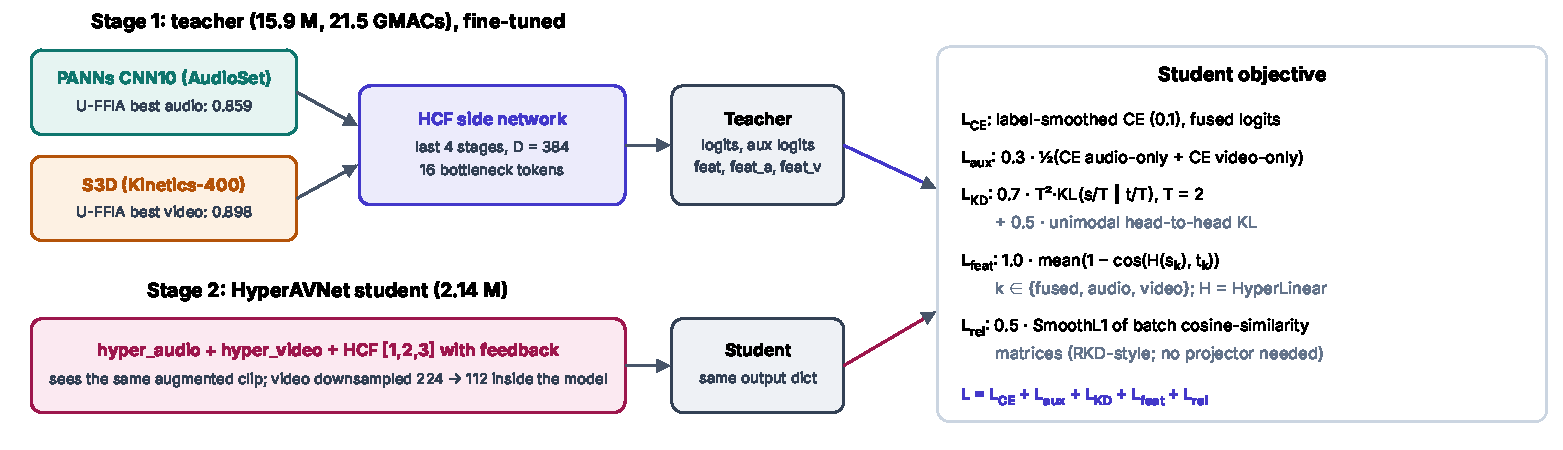
\includegraphics[width=0.92\textwidth]{figures/distillation.pdf}
  \caption{Two-stage training. A teacher built from pretrained audio and video backbones and HCF fusion
  is trained first and frozen. The HyperAVNet student is then trained with the supervised loss plus
  logit-, embedding- and relation-level distillation (Eq.~\eqref{eq:total}).}
  \label{fig:distill}
\end{figure*}

\subsection{Complexity}
\label{sec:complexity}
By Eq.~\eqref{eq:params}, every hypercomplex projection stores $1/n$ of the real parameters. Only the
stems, the depth-wise convolutions, normalisation layers and the final $4$-way classifier stay real.
For the default student ($n=4$), the network has 2.14\,M parameters against 7.88\,M for the identical
real network ($n=1$), and 1.24\,M (octonion) or 0.78\,M (sedenion) for higher algebras. Compute is
1.18\,GMACs per clip for every $n$ (16 frames at $112^{2}$ and 2\,s of audio). The added cost of a
fusion stage is about 0.17\,M parameters and under 0.02\,GMACs.
 in any paper.
%  Requires: amsmath, amssymb, bm, booktabs, graphicx, (cleveref optional).
% ============================================================================
\section{Methodology}
\label{sec:method}

\subsection{Problem formulation}
\label{sec:problem}
Each sample of AV-FFIA is a synchronised two-second clip $(\mathbf{x}^{a}, \mathbf{X}^{v})$, where
$\mathbf{x}^{a}\in\mathbb{R}^{L}$ is the hydrophone waveform ($L = 2f_s$, $f_s = 64$\,kHz) and
$\mathbf{X}^{v}\in[0,1]^{3\times T\times H\times W}$ holds $T$ RGB frames sampled uniformly from the
overhead camera. The label $y\in\mathcal{Y}=\{\textsc{None},\textsc{Weak},\textsc{Medium},\textsc{Strong}\}$
is the feeding intensity. We learn $f_{\theta}:(\mathbf{x}^{a},\mathbf{X}^{v})\mapsto\mathbf{p}\in\Delta^{|\mathcal{Y}|-1}$ with
two goals that pull in opposite directions: high accuracy, robust to the acoustic and visual
corruptions typical of aquaculture (bubbles, pumps, low light, reflections), and a small
parameter and compute budget for on-site deployment.

HyperAVNet (Fig.~\ref{fig:overview}) has four parts. Two hypercomplex backbones map each modality to a
hierarchy of \emph{stage tokens} (Sec.~\ref{sec:backbones}). A set of shared \emph{bottleneck tokens}
is updated by hypercomplex component fusion (HCF) blocks attached at a configurable subset of
stages, with zero-initialised cross-modal feedback into both streams (Secs.~\ref{sec:hcf},~\ref{sec:schedule}).
Fused and unimodal heads produce the predictions (Sec.~\ref{sec:heads}). The model is trained with a
multi-level distillation objective from a pretrained audio-visual teacher (Sec.~\ref{sec:objective}).

\begin{figure*}[t]
  \centering
  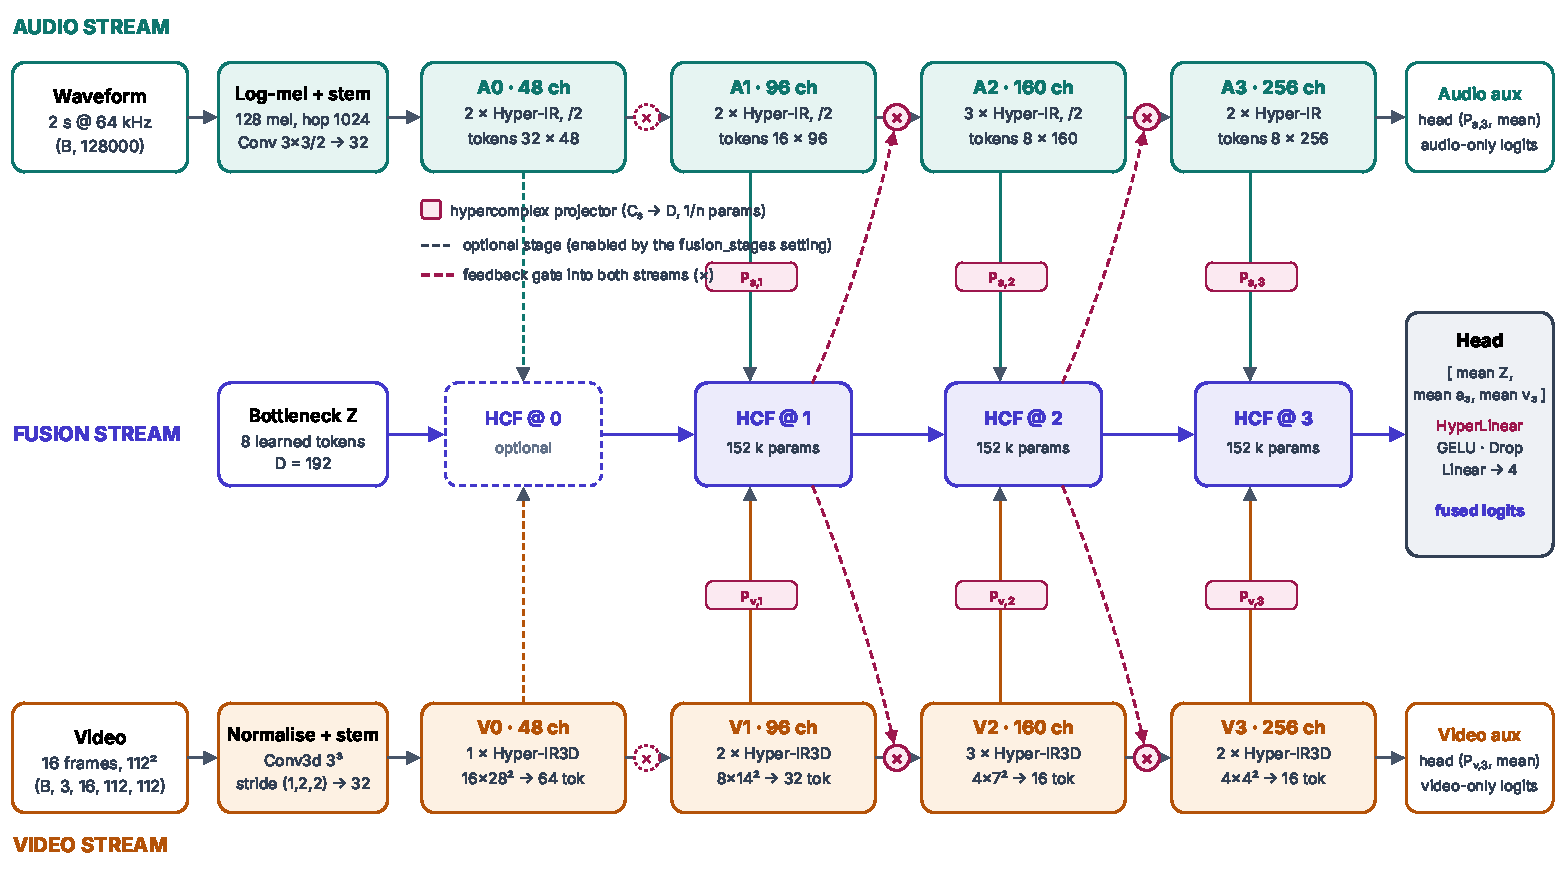
\includegraphics[width=\textwidth]{figures/arch_overview.pdf}
  \caption{HyperAVNet (default configuration: quaternion algebra, fusion stages $\mathcal{S}=\{1,2,3\}$,
  feedback enabled). Stage tokens of the audio and video backbones are projected by hypercomplex
  projectors $P_{a,s}$ and $P_{v,s}$ into a $D$-dimensional fusion space, where HCF blocks update the
  bottleneck tokens $\mathbf{Z}$. After each fused stage $s<S-1$, a zero-initialised gate ($\times$)
  modulates both streams. The classifier reads the pooled bottleneck and the pooled last-stage
  tokens; auxiliary heads supervise each modality on its own. Token shapes are for one 2\,s clip and
  $16\times112^{2}$ frames.}
  \label{fig:overview}
\end{figure*}

\subsection{Hypercomplex layers}
\label{sec:hyper}
Let $\mathbb{A}_n$ be a hypercomplex algebra of dimension $n\in\{2,4,8,16\}$ (complex numbers,
quaternions, octonions, sedenions, obtained by the Cayley--Dickson construction), with basis
$\{e_0,\dots,e_{n-1}\}$ and multiplication table
\begin{equation}
  e_i\,e_j = \sigma_{ij}\, e_{\pi(i,j)},
  \label{eq:table}
\end{equation}
with signs $\sigma_{ij}\in\{-1,+1\}$ and indices $\pi(i,j)\in\{0,\dots,n-1\}$.
A feature vector $\mathbf{x}\in\mathbb{R}^{d_{\mathrm{in}}}$ is split into $n$ components,
$\mathbf{x}=[\mathbf{x}_0;\dots;\mathbf{x}_{n-1}]$ with $\mathbf{x}_j\in\mathbb{R}^{d_{\mathrm{in}}/n}$,
i.e.\ it is read as $\sum_j \mathbf{x}_j e_j$. A hypercomplex weight
$\mathbf{W}=\sum_{k}\mathbf{W}_k e_k$ with real blocks $\mathbf{W}_k\in\mathbb{R}^{(d_{\mathrm{out}}/n)\times(d_{\mathrm{in}}/n)}$
acts on it by the algebra product, which in matrix form is
\begin{equation}
\begin{gathered}
  \mathbf{y}_i = \sum_{j=0}^{n-1} s_{ij}\,\mathbf{W}_{c(i,j)}\,\mathbf{x}_j + \mathbf{b}_i,\\
  \mathbf{K}(\mathbf{W}) = \big[\, s_{ij}\,\mathbf{W}_{c(i,j)} \,\big]_{i,j=0}^{n-1}\in\mathbb{R}^{d_{\mathrm{out}}\times d_{\mathrm{in}}},
\end{gathered}
  \label{eq:hlinear}
\end{equation}
where the block index $c(i,j)$ and sign $s_{ij}$ follow from Eq.~\eqref{eq:table}. For quaternions the
kernel takes the familiar Hamilton form (Fig.~\ref{fig:hamilton}),
\begin{equation}
  \mathbf{K} = \begin{bmatrix}
   \mathbf{W}_0 & \mathbf{W}_1 & \mathbf{W}_2 & \mathbf{W}_3\\
  -\mathbf{W}_1 & \mathbf{W}_0 & \mathbf{W}_3 & -\mathbf{W}_2\\
  -\mathbf{W}_2 & -\mathbf{W}_3 & \mathbf{W}_0 & \mathbf{W}_1\\
  -\mathbf{W}_3 & \mathbf{W}_2 & -\mathbf{W}_1 & \mathbf{W}_0
  \end{bmatrix}.
  \label{eq:hamilton}
\end{equation}
Every output component is thus a signed combination of \emph{every} input component through one
shared set of $n$ blocks, so the layer has
\begin{equation}
  |\theta_{\mathrm{hyper}}| = \tfrac{1}{n}\,d_{\mathrm{in}}d_{\mathrm{out}} + d_{\mathrm{out}}
  \;\;\text{vs.}\;\;
  |\theta_{\mathrm{real}}| = d_{\mathrm{in}}d_{\mathrm{out}} + d_{\mathrm{out}}
  \label{eq:params}
\end{equation}
parameters. A hypercomplex convolution applies the same block structure to the kernel tensor, with
$\mathbf{W}_k\in\mathbb{R}^{(C_{\mathrm{out}}/n)\times(C_{\mathrm{in}}/n)\times k_1\times\dots}$.
Weights are initialised in polar form: a modulus drawn from a $\chi$ distribution with $n$ degrees of
freedom (scaled by the Glorot variance), a uniform phase, and a unit-norm imaginary direction
\cite{bojesomo2024hypercomplex}. We write $\mathcal{H}_n(\cdot)$ for a hypercomplex linear or
convolutional layer. With $n=1$ it reduces to the real layer, which gives a matched real-valued
ablation with an identical code path.

\paragraph{Deployment.} Building $\mathbf{K}$ in Eq.~\eqref{eq:hlinear} at every forward pass
is only needed while training. After training, every $\mathcal{H}_n$ is \emph{reparameterised} into a
dense layer with weight $\mathbf{K}(\mathbf{W})$. The outputs are identical, and the run-time
overhead of kernel assembly disappears. The hypercomplex structure therefore reduces the number of
stored and optimised parameters (and the model's memory and transmission size) by up to $n\times$,
but \emph{not} the multiply--accumulate count, because $\mathbf{K}$ is dense.

\begin{figure}[t]
  \centering
  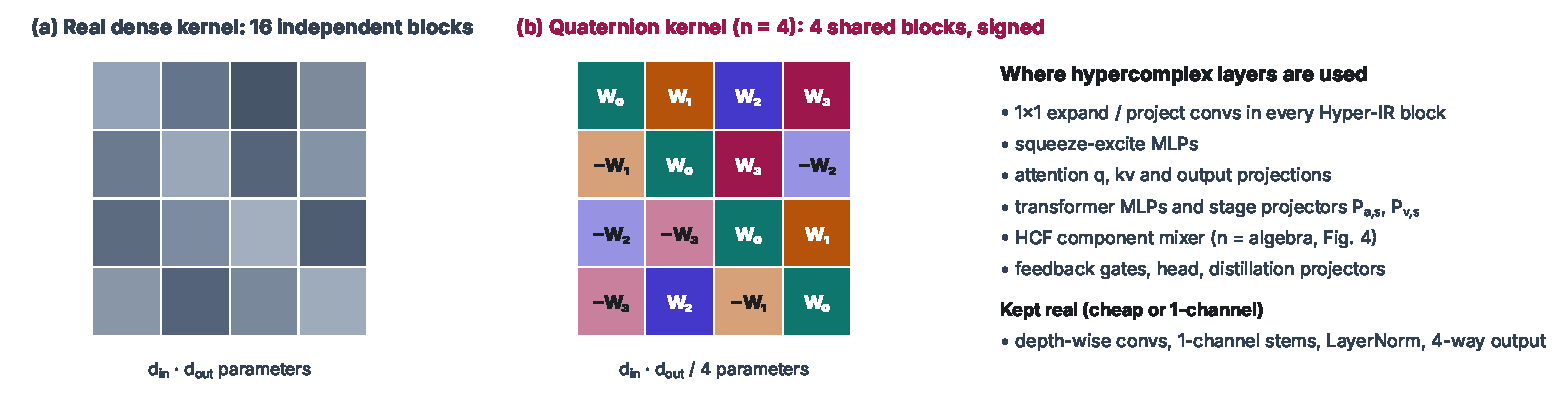
\includegraphics[width=\columnwidth]{figures/hamilton.pdf}
  \caption{Hamilton-product weight sharing. (a) A real kernel has $n^{2}$ independent blocks.
  (b) A quaternion kernel ($n=4$) re-uses four blocks with fixed signs (Eq.~\eqref{eq:hamilton}),
  which cuts the parameter count by $4\times$.}
  \label{fig:hamilton}
\end{figure}

\subsection{Hypercomplex backbones and stage tokens}
\label{sec:backbones}
\paragraph{Hyper-IR block.} Both backbones stack hypercomplex inverted-residual blocks
(Fig.~\ref{fig:hyperir}). For an input $\mathbf{h}\in\mathbb{R}^{C\times\Omega}$ ($\Omega$ is the 2-D
time--frequency grid for audio and the 3-D space--time grid for video) and expansion ratio $r=4$:
\begin{equation}
\begin{aligned}
  \mathbf{u} &= \operatorname{SiLU}\big(\operatorname{BN}(\mathcal{H}_n^{1\times1}(\mathbf{h}))\big)\in\mathbb{R}^{rC\times\Omega},\\
  \mathbf{v} &= \operatorname{SiLU}\big(\operatorname{BN}(\operatorname{DWConv}_{3}(\mathbf{u}))\big),\\
  \mathbf{w} &= \mathbf{v}\odot\sigma\big(\mathcal{H}_n(\operatorname{SiLU}(\mathcal{H}_n(\operatorname{GAP}(\mathbf{v}))))\big),\\
  \mathbf{h}' &= \mathbf{h} + \operatorname{DropPath}\big(\operatorname{BN}(\mathcal{H}_n^{1\times1}(\mathbf{w}))\big).
\end{aligned}
  \label{eq:hyperir}
\end{equation}
The two point-wise convolutions hold almost all of a block's parameters, so they are hypercomplex. The
depth-wise convolution stays real; it accounts for about 1\% of the parameters. The residual is used
when the shape is preserved.

\paragraph{Audio stream.} The waveform is converted to a log-mel spectrogram with the U-FFIA settings
(Hann window 2048, hop 1024, 128 mel bins at 64\,kHz, so a 2\,s clip gives $128\times126$),
normalised per mel bin by batch normalisation and augmented with SpecAugment during training. A
$3{\times}3$ stride-2 stem is followed by four Hyper-IR stages $s=0,\dots,3$ with widths
$(48,96,160,256)$ and depths $(2,2,3,2)$. A stage map $\mathbf{h}^{a}_{s}\in\mathbb{R}^{C_s\times T_s\times F_s}$
becomes time tokens by pooling over frequency:
\begin{equation}
  \mathbf{a}_s = \big[\operatorname{mean}_{F}(\mathbf{h}^{a}_s) + \operatorname{max}_{F}(\mathbf{h}^{a}_s)\big]^{\top}\in\mathbb{R}^{T_s\times C_s}.
  \label{eq:audiotokens}
\end{equation}
The max term keeps the short impulsive transients of feeding (chewing, tail slaps).

\paragraph{Video stream.} The frames are normalised and passed through a $3{\times}3{\times}3$ stem
(spatial stride 2) and four 3-D Hyper-IR stages of the same widths, with depths $(1,2,3,2)$ and
strides $(1,2,2)$, $(2,2,2)$, $(2,2,2)$, $(1,2,2)$. A stage map
$\mathbf{h}^{v}_{s}\in\mathbb{R}^{C_s\times T_s\times H_s\times W_s}$ is pooled to a $2\times2$ spatial grid
per time step, $\mathbf{v}_s\in\mathbb{R}^{4T_s\times C_s}$. This keeps coarse location (where the fish
aggregate) at a small token count.

\begin{figure}[t]
  \centering
  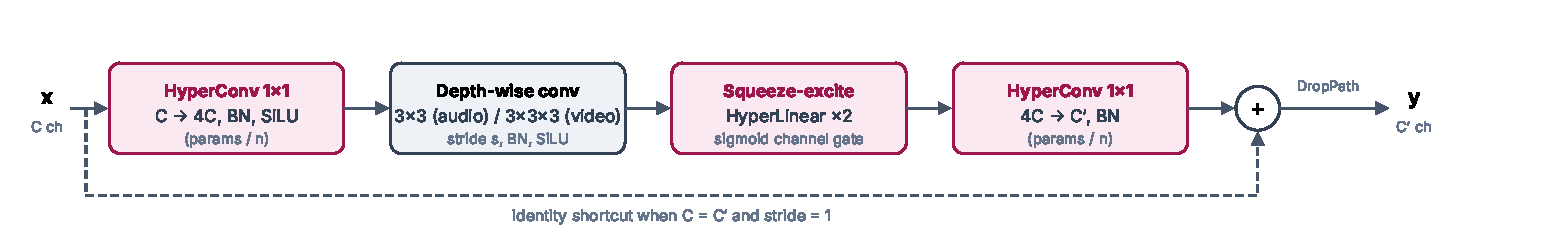
\includegraphics[width=\columnwidth]{figures/hyper_ir.pdf}
  \caption{Hypercomplex inverted-residual (Hyper-IR) block, Eq.~\eqref{eq:hyperir}. Hypercomplex
  layers are shaded; the depth-wise convolution is real.}
  \label{fig:hyperir}
\end{figure}

\paragraph{Pretrained backbones.} Any pretrained network can replace a student backbone if it exposes
four stages in the same token format. We use this for the teachers and for the teacher ablation
(Sec.~\ref{sec:setup}): PANNs CNN10/CNN14~\cite{kong2020panns}, EfficientAT~\cite{schmid2023efficientat},
AST~\cite{gong2021ast}, S3D~\cite{xie2018s3d}, X3D~\cite{feichtenhofer2020x3d},
MoViNet~\cite{kondratyuk2021movinets} and VideoMAE~\cite{tong2022videomae}. Their intermediate layers
supply the stage tokens.

\subsection{Hypercomplex component fusion}
\label{sec:hcf}
\paragraph{Projection.} Stage tokens are mapped into a shared $D$-dimensional space by hypercomplex
projectors with a learned modality embedding:
\begin{equation}
  \mathbf{A}_s = \operatorname{LN}\!\big(\mathcal{H}_n(\mathbf{a}_s)\big) + \mathbf{m}^{a},\qquad
  \mathbf{V}_s = \operatorname{LN}\!\big(\mathcal{H}_n(\mathbf{v}_s)\big) + \mathbf{m}^{v}.
  \label{eq:proj}
\end{equation}

\paragraph{Bottleneck state.} The fused representation lives in $N_b$ learned bottleneck tokens
$\mathbf{Z}\in\mathbb{R}^{N_b\times D}$ (we use $N_b=8$, $D=192$), shared across stages.

\paragraph{HCF block.} At a fusion stage $s$, the bottleneck first reads each modality with its own
hypercomplex cross-attention:
\begin{equation}
\begin{aligned}
  \mathbf{Z}^{a} &= \mathbf{Z} + \operatorname{XAttn}_{n}\big(\operatorname{LN}\mathbf{Z},\,\operatorname{LN}\mathbf{A}_s\big),\\
  \mathbf{Z}^{v} &= \mathbf{Z} + \operatorname{XAttn}_{n}\big(\operatorname{LN}\mathbf{Z},\,\operatorname{LN}\mathbf{V}_s\big),
\end{aligned}
  \label{eq:xattn}
\end{equation}
where $\operatorname{XAttn}_n$ is multi-head attention whose query, key, value and output projections
are hypercomplex (shown for one head of width $d_h$):
\begin{equation*}
  \operatorname{XAttn}_n(\mathbf{Q},\mathbf{C})=\mathcal{H}_n\Big(\operatorname{softmax}\Big(\tfrac{\mathcal{H}_n(\mathbf{Q})\,\mathcal{H}_n(\mathbf{C})^{\top}}{\sqrt{d_h}}\Big)\mathcal{H}_n(\mathbf{C})\Big).
\end{equation*} The shared
state, the two modality views and their interaction then form the components of one element of
$\mathbb{A}_m$:
\begin{equation}
  \mathbf{q} = \mathbf{Z}\,e_0 + \mathbf{Z}^{a}\,e_1 + \mathbf{Z}^{v}\,e_2 + \big(\hat{\mathbf{Z}}^{a}\odot\hat{\mathbf{Z}}^{v}\big)\,e_3,
  \label{eq:components}
\end{equation}
for $m=4$,
with $\hat{\cdot}=\operatorname{LN}(\cdot)$. The octonion variant ($m=8$) appends
$(\mathbf{Z}^{a}-\mathbf{Z}^{v})e_4$, $(\hat{\mathbf{Z}}\odot\hat{\mathbf{Z}}^{a})e_5$,
$(\hat{\mathbf{Z}}\odot\hat{\mathbf{Z}}^{v})e_6$ and
$(\hat{\mathbf{Z}}\odot\hat{\mathbf{Z}}^{a}\odot\hat{\mathbf{Z}}^{v})e_7$; the complex variant ($m=2$) uses
$(\mathbf{Z}^{a},\mathbf{Z}^{v})$. The components are mixed by a single Hamilton product, followed by a
hypercomplex MLP:
\begin{equation}
\begin{aligned}
  \mathbf{Z} &\leftarrow \mathbf{Z} + \boldsymbol{\gamma}_1\odot \mathcal{H}_m(\mathbf{q}),\\
  \mathbf{Z} &\leftarrow \mathbf{Z} + \boldsymbol{\gamma}_2\odot \operatorname{MLP}_n(\operatorname{LN}\mathbf{Z}),
\end{aligned}
  \label{eq:mix}
\end{equation}
where $\mathcal{H}_m:\mathbb{R}^{mD}\to\mathbb{R}^{D}$ is a hypercomplex linear layer of algebra
$\mathbb{A}_m$ and $\boldsymbol{\gamma}_{1,2}$ are LayerScale vectors~\cite{touvron2021cait}, initialised to
$10^{-2}$. By Eq.~\eqref{eq:hlinear}, each output component of $\mathcal{H}_m$ is a signed mixture of
the shared state, both modality views and their multiplicative agreement, all through one set of
$m$ blocks. The mixer has $D^{2}$ parameters \emph{for every} $m$, against $mD^{2}$ for a dense mixer, so
the octonion variant adds four interaction terms at no parameter cost. Unlike attention bottlenecks
that attend to the modalities one after the other~\cite{nagrani2021mbt}, HCF reads both modalities
in parallel and combines them in one algebraic product (Fig.~\ref{fig:hcf}).

\begin{figure*}[t]
  \centering
  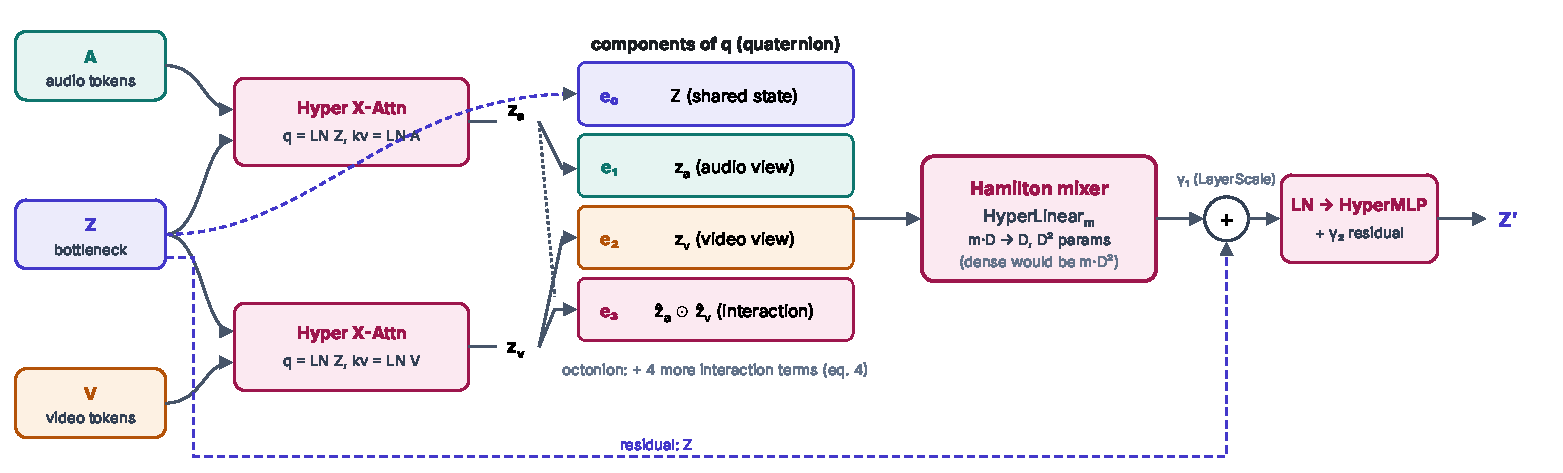
\includegraphics[width=0.9\textwidth]{figures/hcf_block.pdf}
  \caption{Hypercomplex component fusion (HCF), Eqs.~\eqref{eq:xattn}--\eqref{eq:mix}. The modality
  views and their interaction are the components of one quaternion and are mixed by a single
  Hamilton product.}
  \label{fig:hcf}
\end{figure*}

\subsection{Deep-to-early fusion schedule with cross-modal feedback}
\label{sec:schedule}
The set $\mathcal{S}\subseteq\{0,\dots,S-1\}$ selects the stages at which an HCF block is attached:
\begin{equation}
  \mathbf{Z}^{(s+1)} = \begin{cases}\operatorname{HCF}_s\big(\mathbf{Z}^{(s)},\mathbf{A}_s,\mathbf{V}_s\big), & s\in\mathcal{S},\\ \mathbf{Z}^{(s)}, & \text{otherwise,}\end{cases}
  \label{eq:schedule}
\end{equation}
with $\mathbf{Z}^{(0)}=\mathbf{Z}_{\mathrm{init}}$ the learned bottleneck tokens.
Varying $\mathcal{S}$ from $\{S-1\}$ (late fusion) through $\{S-2,S-1\}$ and so on to $\{0,\dots,S-1\}$
gives a controlled \emph{deep-to-early} study of where audio--visual fusion helps. Because the student
backbones are executed stage by stage, the fused state is also fed back into both streams after each
fused stage $s<S-1$:
\begin{equation}
  \mathbf{h}^{m}_s \leftarrow \mathbf{h}^{m}_s\odot\big(1+\tanh(\mathcal{G}^{m}_s\,\bar{\mathbf{z}}^{(s+1)})\big),\quad m\in\{a,v\},
  \label{eq:feedback}
\end{equation}
where $\bar{\mathbf{z}}=\operatorname{mean}_{N_b}(\mathbf{Z})$, the gates
$\mathcal{G}^{m}_s$ are hypercomplex linear maps $\mathbb{R}^{D}\to\mathbb{R}^{C_s}$, and the
product broadcasts over $\Omega$. The gates are \emph{initialised to zero}, so training starts exactly
at the feedback-free model. The network then learns how strongly each modality should condition the
other's later features. This is genuine early fusion, as opposed to fusing independently computed
features.

\subsection{Prediction heads and modality dropout}
\label{sec:heads}
With $\bar{\mathbf{z}}=\operatorname{mean}(\operatorname{LN}\mathbf{Z}^{(S)})$,
$\bar{\mathbf{a}}=\operatorname{mean}(\operatorname{LN}\mathbf{A}_{S-1})$ and
$\bar{\mathbf{v}}=\operatorname{mean}(\operatorname{LN}\mathbf{V}_{S-1})$, the fused and auxiliary logits are
\begin{equation}
\begin{gathered}
  \boldsymbol{\ell} = \mathbf{W}_o\,\operatorname{GELU}\big(\mathcal{H}_n[\bar{\mathbf{z}};\,\mu_a\bar{\mathbf{a}};\,\mu_v\bar{\mathbf{v}}]\big),\\
  \boldsymbol{\ell}^{a} = \mathbf{W}_a\bar{\mathbf{a}},\qquad \boldsymbol{\ell}^{v} = \mathbf{W}_v\bar{\mathbf{v}}.
\end{gathered}
  \label{eq:heads}
\end{equation}
Here $\mu_a,\mu_v\in\{0,1\}$ are per-sample modality masks. During training,
$(\mu_a,\mu_v)=(0,1)$ with probability $p$, $(1,0)$ with probability $p$, and $(1,1)$ otherwise. In the
notation of~\cite{cui2024uffia}, $p_{av}=1-2p$ and $p_a=p_v=p$. The same mask multiplies every fusion
input $\mathbf{A}_s,\mathbf{V}_s$, so a dropped modality is absent everywhere. The auxiliary heads always see
their own modality, which keeps both branches trained regardless of $p$. At test time, forcing
$\mu_a=0$ or $\mu_v=0$ evaluates the model with a missing modality.

\subsection{Training objective and multi-level distillation}
\label{sec:objective}
The supervised loss combines label-smoothed cross-entropy on the fused logits with the two
auxiliary terms:
\begin{equation}
  \mathcal{L}_{\mathrm{sup}} = \operatorname{CE}_{\epsilon}(\boldsymbol{\ell},y)
   + \tfrac{\lambda_{\mathrm{aux}}}{2}\!\!\sum_{m\in\{a,v\}}\!\!\operatorname{CE}_{\epsilon}(\boldsymbol{\ell}^{m},y).
  \label{eq:sup}
\end{equation}
A frozen teacher $g$ with the same output structure (pretrained backbones and HCF fusion) provides
three further signals. At the \emph{logit level}, with temperature $\tau$:
\begin{equation}
  \mathcal{L}_{\mathrm{KD}} = \tau^{2}\,\mathrm{KL}\big(\boldsymbol{\ell}^{g}\,\|\,\boldsymbol{\ell}\big)_{\tau}
   + \tfrac{\lambda_{u}\tau^{2}}{2}\!\!\sum_{m\in\{a,v\}}\!\!\mathrm{KL}\big(\boldsymbol{\ell}^{g,m}\,\|\,\boldsymbol{\ell}^{m}\big)_{\tau},
  \label{eq:kd}
\end{equation}
with $\mathrm{KL}(\mathbf{u}\,\|\,\mathbf{w})_{\tau}=\mathrm{KL}\big(\operatorname{softmax}(\mathbf{u}/\tau)\,\|\,\operatorname{softmax}(\mathbf{w}/\tau)\big)$,
which distils each unimodal head from its counterpart in the teacher. U-FFIA's variant~\cite{cui2024uffia}
softens only the teacher, $\mathrm{KL}(\operatorname{softmax}(\boldsymbol{\ell}^{g}/\tau)\,\|\,\operatorname{softmax}(\boldsymbol{\ell}))$,
and is evaluated as an ablation. At the \emph{embedding level}, small hypercomplex projectors
$\mathcal{P}_k$ align the student's pooled embeddings with the teacher's:
\begin{equation}
  \mathcal{L}_{\mathrm{feat}} = \tfrac{1}{3}\!\!\sum_{k\in\{\bar{\mathbf{z}},\bar{\mathbf{a}},\bar{\mathbf{v}}\}}\!\!
  \big(1-\cos(\mathcal{P}_k(k),\,k^{g})\big).
  \label{eq:feat}
\end{equation}
At the \emph{relation level}~\cite{park2019rkd}, the within-batch similarity structure of the fused
embeddings is matched:
\begin{equation}
  \mathcal{L}_{\mathrm{rel}} = \operatorname{SmoothL1}\big(\mathbf{R}(\bar{\mathbf{z}}_{1:B}),\,\mathbf{R}(\bar{\mathbf{z}}^{g}_{1:B})\big),
  \label{eq:rel}
\end{equation}
where $\mathbf{R}(\mathbf{U})_{ij}=\mathbf{u}_i^{\top}\mathbf{u}_j/(\|\mathbf{u}_i\|\|\mathbf{u}_j\|)$ is the cosine-similarity matrix of a batch of size $B$.
The full objective is
\begin{equation}
  \mathcal{L} = \mathcal{L}_{\mathrm{sup}} + \alpha\,\mathcal{L}_{\mathrm{KD}} + \beta\,\mathcal{L}_{\mathrm{feat}} + \gamma\,\mathcal{L}_{\mathrm{rel}},
  \label{eq:total}
\end{equation}
with $\epsilon=0.1$, $\lambda_{\mathrm{aux}}=0.3$, $\lambda_u=0.5$, $\tau=2$, $\alpha=0.7$, $\beta=1$ and $\gamma=0.5$.
Training proceeds in two stages: the teacher is trained with $\mathcal{L}_{\mathrm{sup}}$ and frozen, then
the student is trained with Eq.~\eqref{eq:total}.

\begin{figure*}[t]
  \centering
  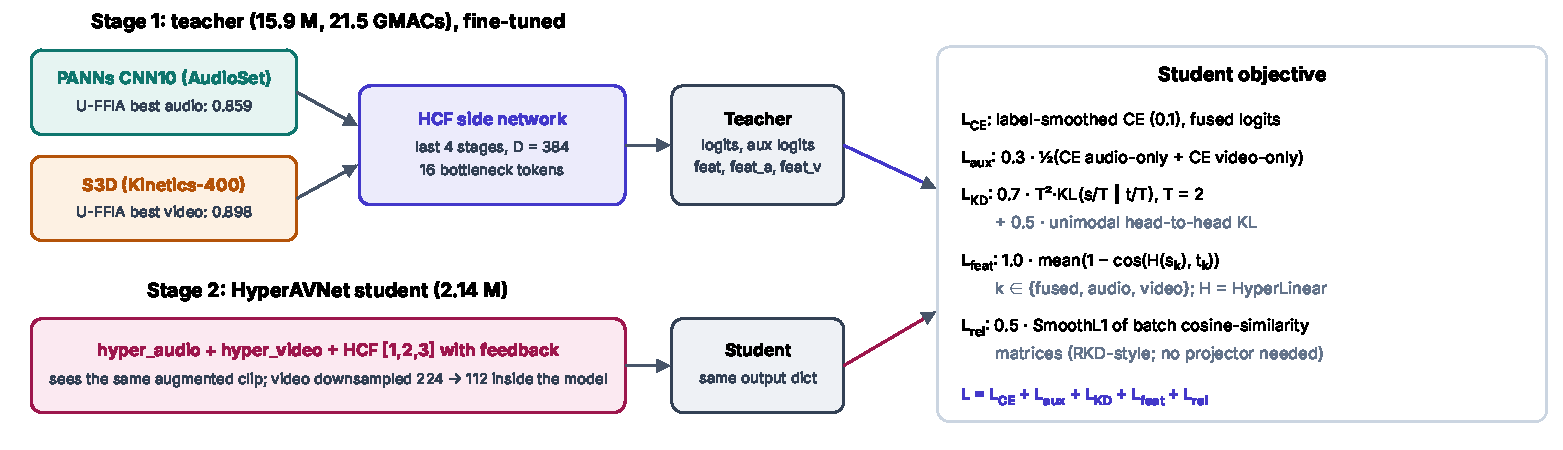
\includegraphics[width=0.92\textwidth]{figures/distillation.pdf}
  \caption{Two-stage training. A teacher built from pretrained audio and video backbones and HCF fusion
  is trained first and frozen. The HyperAVNet student is then trained with the supervised loss plus
  logit-, embedding- and relation-level distillation (Eq.~\eqref{eq:total}).}
  \label{fig:distill}
\end{figure*}

\subsection{Complexity}
\label{sec:complexity}
By Eq.~\eqref{eq:params}, every hypercomplex projection stores $1/n$ of the real parameters. Only the
stems, the depth-wise convolutions, normalisation layers and the final $4$-way classifier stay real.
For the default student ($n=4$), the network has 2.14\,M parameters against 7.88\,M for the identical
real network ($n=1$), and 1.24\,M (octonion) or 0.78\,M (sedenion) for higher algebras. Compute is
1.18\,GMACs per clip for every $n$ (16 frames at $112^{2}$ and 2\,s of audio). The added cost of a
fusion stage is about 0.17\,M parameters and under 0.02\,GMACs.
 in any paper.
%  Requires: amsmath, amssymb, bm, booktabs, graphicx, (cleveref optional).
% ============================================================================
\section{Methodology}
\label{sec:method}

\subsection{Problem formulation}
\label{sec:problem}
Each sample of AV-FFIA is a synchronised two-second clip $(\mathbf{x}^{a}, \mathbf{X}^{v})$, where
$\mathbf{x}^{a}\in\mathbb{R}^{L}$ is the hydrophone waveform ($L = 2f_s$, $f_s = 64$\,kHz) and
$\mathbf{X}^{v}\in[0,1]^{3\times T\times H\times W}$ holds $T$ RGB frames sampled uniformly from the
overhead camera. The label $y\in\mathcal{Y}=\{\textsc{None},\textsc{Weak},\textsc{Medium},\textsc{Strong}\}$
is the feeding intensity. We learn $f_{\theta}:(\mathbf{x}^{a},\mathbf{X}^{v})\mapsto\mathbf{p}\in\Delta^{|\mathcal{Y}|-1}$ with
two goals that pull in opposite directions: high accuracy, robust to the acoustic and visual
corruptions typical of aquaculture (bubbles, pumps, low light, reflections), and a small
parameter and compute budget for on-site deployment.

HyperAVNet (Fig.~\ref{fig:overview}) has four parts. Two hypercomplex backbones map each modality to a
hierarchy of \emph{stage tokens} (Sec.~\ref{sec:backbones}). A set of shared \emph{bottleneck tokens}
is updated by hypercomplex component fusion (HCF) blocks attached at a configurable subset of
stages, with zero-initialised cross-modal feedback into both streams (Secs.~\ref{sec:hcf},~\ref{sec:schedule}).
Fused and unimodal heads produce the predictions (Sec.~\ref{sec:heads}). The model is trained with a
multi-level distillation objective from a pretrained audio-visual teacher (Sec.~\ref{sec:objective}).

\begin{figure*}[t]
  \centering
  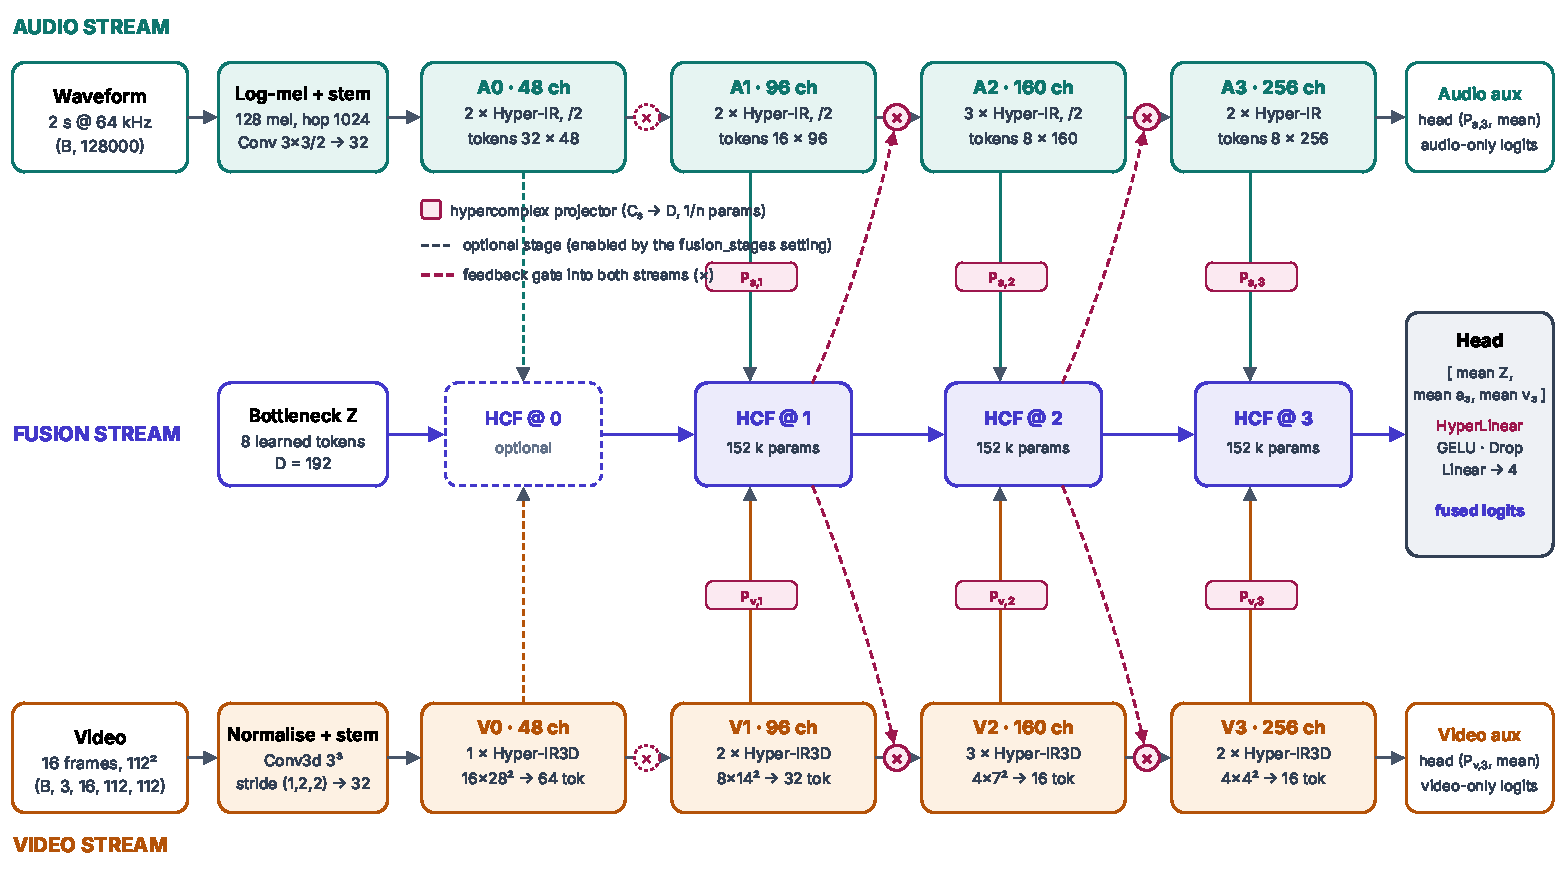
\includegraphics[width=\textwidth]{figures/arch_overview.pdf}
  \caption{HyperAVNet (default configuration: quaternion algebra, fusion stages $\mathcal{S}=\{1,2,3\}$,
  feedback enabled). Stage tokens of the audio and video backbones are projected by hypercomplex
  projectors $P_{a,s}$ and $P_{v,s}$ into a $D$-dimensional fusion space, where HCF blocks update the
  bottleneck tokens $\mathbf{Z}$. After each fused stage $s<S-1$, a zero-initialised gate ($\times$)
  modulates both streams. The classifier reads the pooled bottleneck and the pooled last-stage
  tokens; auxiliary heads supervise each modality on its own. Token shapes are for one 2\,s clip and
  $16\times112^{2}$ frames.}
  \label{fig:overview}
\end{figure*}

\subsection{Hypercomplex layers}
\label{sec:hyper}
Let $\mathbb{A}_n$ be a hypercomplex algebra of dimension $n\in\{2,4,8,16\}$ (complex numbers,
quaternions, octonions, sedenions, obtained by the Cayley--Dickson construction), with basis
$\{e_0,\dots,e_{n-1}\}$ and multiplication table
\begin{equation}
  e_i\,e_j = \sigma_{ij}\, e_{\pi(i,j)},
  \label{eq:table}
\end{equation}
with signs $\sigma_{ij}\in\{-1,+1\}$ and indices $\pi(i,j)\in\{0,\dots,n-1\}$.
A feature vector $\mathbf{x}\in\mathbb{R}^{d_{\mathrm{in}}}$ is split into $n$ components,
$\mathbf{x}=[\mathbf{x}_0;\dots;\mathbf{x}_{n-1}]$ with $\mathbf{x}_j\in\mathbb{R}^{d_{\mathrm{in}}/n}$,
i.e.\ it is read as $\sum_j \mathbf{x}_j e_j$. A hypercomplex weight
$\mathbf{W}=\sum_{k}\mathbf{W}_k e_k$ with real blocks $\mathbf{W}_k\in\mathbb{R}^{(d_{\mathrm{out}}/n)\times(d_{\mathrm{in}}/n)}$
acts on it by the algebra product, which in matrix form is
\begin{equation}
\begin{gathered}
  \mathbf{y}_i = \sum_{j=0}^{n-1} s_{ij}\,\mathbf{W}_{c(i,j)}\,\mathbf{x}_j + \mathbf{b}_i,\\
  \mathbf{K}(\mathbf{W}) = \big[\, s_{ij}\,\mathbf{W}_{c(i,j)} \,\big]_{i,j=0}^{n-1}\in\mathbb{R}^{d_{\mathrm{out}}\times d_{\mathrm{in}}},
\end{gathered}
  \label{eq:hlinear}
\end{equation}
where the block index $c(i,j)$ and sign $s_{ij}$ follow from Eq.~\eqref{eq:table}. For quaternions the
kernel takes the familiar Hamilton form (Fig.~\ref{fig:hamilton}),
\begin{equation}
  \mathbf{K} = \begin{bmatrix}
   \mathbf{W}_0 & \mathbf{W}_1 & \mathbf{W}_2 & \mathbf{W}_3\\
  -\mathbf{W}_1 & \mathbf{W}_0 & \mathbf{W}_3 & -\mathbf{W}_2\\
  -\mathbf{W}_2 & -\mathbf{W}_3 & \mathbf{W}_0 & \mathbf{W}_1\\
  -\mathbf{W}_3 & \mathbf{W}_2 & -\mathbf{W}_1 & \mathbf{W}_0
  \end{bmatrix}.
  \label{eq:hamilton}
\end{equation}
Every output component is thus a signed combination of \emph{every} input component through one
shared set of $n$ blocks, so the layer has
\begin{equation}
  |\theta_{\mathrm{hyper}}| = \tfrac{1}{n}\,d_{\mathrm{in}}d_{\mathrm{out}} + d_{\mathrm{out}}
  \;\;\text{vs.}\;\;
  |\theta_{\mathrm{real}}| = d_{\mathrm{in}}d_{\mathrm{out}} + d_{\mathrm{out}}
  \label{eq:params}
\end{equation}
parameters. A hypercomplex convolution applies the same block structure to the kernel tensor, with
$\mathbf{W}_k\in\mathbb{R}^{(C_{\mathrm{out}}/n)\times(C_{\mathrm{in}}/n)\times k_1\times\dots}$.
Weights are initialised in polar form: a modulus drawn from a $\chi$ distribution with $n$ degrees of
freedom (scaled by the Glorot variance), a uniform phase, and a unit-norm imaginary direction
\cite{bojesomo2024hypercomplex}. We write $\mathcal{H}_n(\cdot)$ for a hypercomplex linear or
convolutional layer. With $n=1$ it reduces to the real layer, which gives a matched real-valued
ablation with an identical code path.

\paragraph{Deployment.} Building $\mathbf{K}$ in Eq.~\eqref{eq:hlinear} at every forward pass
is only needed while training. After training, every $\mathcal{H}_n$ is \emph{reparameterised} into a
dense layer with weight $\mathbf{K}(\mathbf{W})$. The outputs are identical, and the run-time
overhead of kernel assembly disappears. The hypercomplex structure therefore reduces the number of
stored and optimised parameters (and the model's memory and transmission size) by up to $n\times$,
but \emph{not} the multiply--accumulate count, because $\mathbf{K}$ is dense.

\begin{figure}[t]
  \centering
  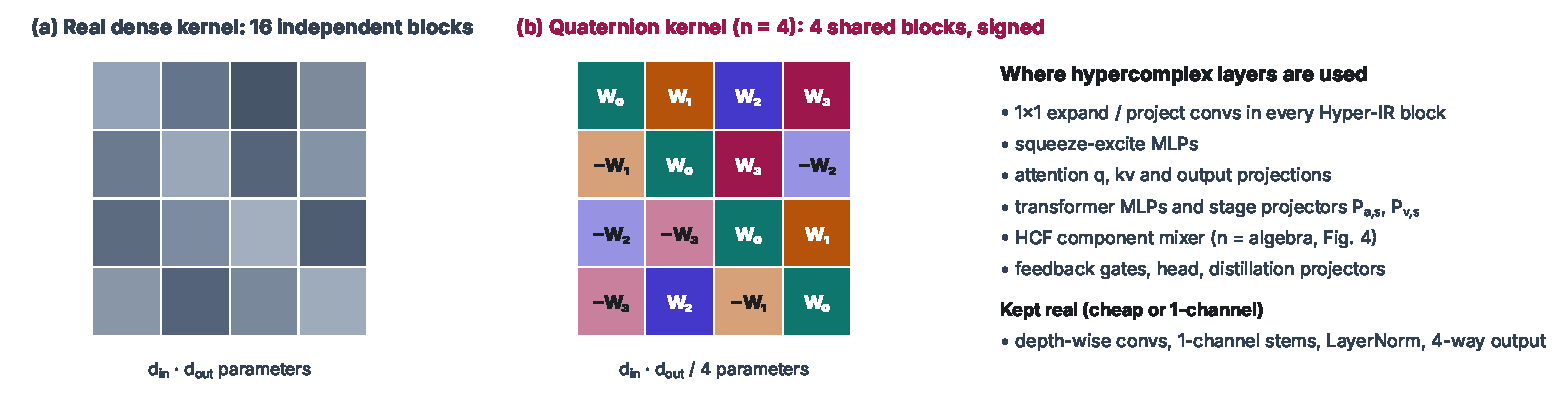
\includegraphics[width=\columnwidth]{figures/hamilton.pdf}
  \caption{Hamilton-product weight sharing. (a) A real kernel has $n^{2}$ independent blocks.
  (b) A quaternion kernel ($n=4$) re-uses four blocks with fixed signs (Eq.~\eqref{eq:hamilton}),
  which cuts the parameter count by $4\times$.}
  \label{fig:hamilton}
\end{figure}

\subsection{Hypercomplex backbones and stage tokens}
\label{sec:backbones}
\paragraph{Hyper-IR block.} Both backbones stack hypercomplex inverted-residual blocks
(Fig.~\ref{fig:hyperir}). For an input $\mathbf{h}\in\mathbb{R}^{C\times\Omega}$ ($\Omega$ is the 2-D
time--frequency grid for audio and the 3-D space--time grid for video) and expansion ratio $r=4$:
\begin{equation}
\begin{aligned}
  \mathbf{u} &= \operatorname{SiLU}\big(\operatorname{BN}(\mathcal{H}_n^{1\times1}(\mathbf{h}))\big)\in\mathbb{R}^{rC\times\Omega},\\
  \mathbf{v} &= \operatorname{SiLU}\big(\operatorname{BN}(\operatorname{DWConv}_{3}(\mathbf{u}))\big),\\
  \mathbf{w} &= \mathbf{v}\odot\sigma\big(\mathcal{H}_n(\operatorname{SiLU}(\mathcal{H}_n(\operatorname{GAP}(\mathbf{v}))))\big),\\
  \mathbf{h}' &= \mathbf{h} + \operatorname{DropPath}\big(\operatorname{BN}(\mathcal{H}_n^{1\times1}(\mathbf{w}))\big).
\end{aligned}
  \label{eq:hyperir}
\end{equation}
The two point-wise convolutions hold almost all of a block's parameters, so they are hypercomplex. The
depth-wise convolution stays real; it accounts for about 1\% of the parameters. The residual is used
when the shape is preserved.

\paragraph{Audio stream.} The waveform is converted to a log-mel spectrogram with the U-FFIA settings
(Hann window 2048, hop 1024, 128 mel bins at 64\,kHz, so a 2\,s clip gives $128\times126$),
normalised per mel bin by batch normalisation and augmented with SpecAugment during training. A
$3{\times}3$ stride-2 stem is followed by four Hyper-IR stages $s=0,\dots,3$ with widths
$(48,96,160,256)$ and depths $(2,2,3,2)$. A stage map $\mathbf{h}^{a}_{s}\in\mathbb{R}^{C_s\times T_s\times F_s}$
becomes time tokens by pooling over frequency:
\begin{equation}
  \mathbf{a}_s = \big[\operatorname{mean}_{F}(\mathbf{h}^{a}_s) + \operatorname{max}_{F}(\mathbf{h}^{a}_s)\big]^{\top}\in\mathbb{R}^{T_s\times C_s}.
  \label{eq:audiotokens}
\end{equation}
The max term keeps the short impulsive transients of feeding (chewing, tail slaps).

\paragraph{Video stream.} The frames are normalised and passed through a $3{\times}3{\times}3$ stem
(spatial stride 2) and four 3-D Hyper-IR stages of the same widths, with depths $(1,2,3,2)$ and
strides $(1,2,2)$, $(2,2,2)$, $(2,2,2)$, $(1,2,2)$. A stage map
$\mathbf{h}^{v}_{s}\in\mathbb{R}^{C_s\times T_s\times H_s\times W_s}$ is pooled to a $2\times2$ spatial grid
per time step, $\mathbf{v}_s\in\mathbb{R}^{4T_s\times C_s}$. This keeps coarse location (where the fish
aggregate) at a small token count.

\begin{figure}[t]
  \centering
  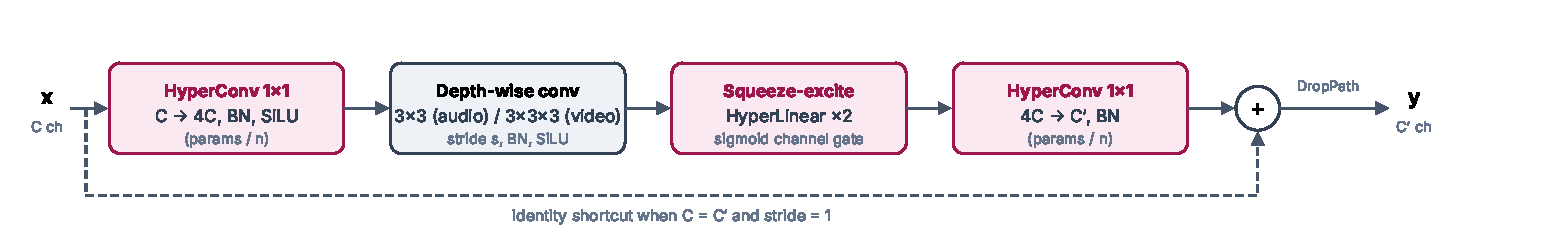
\includegraphics[width=\columnwidth]{figures/hyper_ir.pdf}
  \caption{Hypercomplex inverted-residual (Hyper-IR) block, Eq.~\eqref{eq:hyperir}. Hypercomplex
  layers are shaded; the depth-wise convolution is real.}
  \label{fig:hyperir}
\end{figure}

\paragraph{Pretrained backbones.} Any pretrained network can replace a student backbone if it exposes
four stages in the same token format. We use this for the teachers and for the teacher ablation
(Sec.~\ref{sec:setup}): PANNs CNN10/CNN14~\cite{kong2020panns}, EfficientAT~\cite{schmid2023efficientat},
AST~\cite{gong2021ast}, S3D~\cite{xie2018s3d}, X3D~\cite{feichtenhofer2020x3d},
MoViNet~\cite{kondratyuk2021movinets} and VideoMAE~\cite{tong2022videomae}. Their intermediate layers
supply the stage tokens.

\subsection{Hypercomplex component fusion}
\label{sec:hcf}
\paragraph{Projection.} Stage tokens are mapped into a shared $D$-dimensional space by hypercomplex
projectors with a learned modality embedding:
\begin{equation}
  \mathbf{A}_s = \operatorname{LN}\!\big(\mathcal{H}_n(\mathbf{a}_s)\big) + \mathbf{m}^{a},\qquad
  \mathbf{V}_s = \operatorname{LN}\!\big(\mathcal{H}_n(\mathbf{v}_s)\big) + \mathbf{m}^{v}.
  \label{eq:proj}
\end{equation}

\paragraph{Bottleneck state.} The fused representation lives in $N_b$ learned bottleneck tokens
$\mathbf{Z}\in\mathbb{R}^{N_b\times D}$ (we use $N_b=8$, $D=192$), shared across stages.

\paragraph{HCF block.} At a fusion stage $s$, the bottleneck first reads each modality with its own
hypercomplex cross-attention:
\begin{equation}
\begin{aligned}
  \mathbf{Z}^{a} &= \mathbf{Z} + \operatorname{XAttn}_{n}\big(\operatorname{LN}\mathbf{Z},\,\operatorname{LN}\mathbf{A}_s\big),\\
  \mathbf{Z}^{v} &= \mathbf{Z} + \operatorname{XAttn}_{n}\big(\operatorname{LN}\mathbf{Z},\,\operatorname{LN}\mathbf{V}_s\big),
\end{aligned}
  \label{eq:xattn}
\end{equation}
where $\operatorname{XAttn}_n$ is multi-head attention whose query, key, value and output projections
are hypercomplex (shown for one head of width $d_h$):
\begin{equation*}
  \operatorname{XAttn}_n(\mathbf{Q},\mathbf{C})=\mathcal{H}_n\Big(\operatorname{softmax}\Big(\tfrac{\mathcal{H}_n(\mathbf{Q})\,\mathcal{H}_n(\mathbf{C})^{\top}}{\sqrt{d_h}}\Big)\mathcal{H}_n(\mathbf{C})\Big).
\end{equation*} The shared
state, the two modality views and their interaction then form the components of one element of
$\mathbb{A}_m$:
\begin{equation}
  \mathbf{q} = \mathbf{Z}\,e_0 + \mathbf{Z}^{a}\,e_1 + \mathbf{Z}^{v}\,e_2 + \big(\hat{\mathbf{Z}}^{a}\odot\hat{\mathbf{Z}}^{v}\big)\,e_3,
  \label{eq:components}
\end{equation}
for $m=4$,
with $\hat{\cdot}=\operatorname{LN}(\cdot)$. The octonion variant ($m=8$) appends
$(\mathbf{Z}^{a}-\mathbf{Z}^{v})e_4$, $(\hat{\mathbf{Z}}\odot\hat{\mathbf{Z}}^{a})e_5$,
$(\hat{\mathbf{Z}}\odot\hat{\mathbf{Z}}^{v})e_6$ and
$(\hat{\mathbf{Z}}\odot\hat{\mathbf{Z}}^{a}\odot\hat{\mathbf{Z}}^{v})e_7$; the complex variant ($m=2$) uses
$(\mathbf{Z}^{a},\mathbf{Z}^{v})$. The components are mixed by a single Hamilton product, followed by a
hypercomplex MLP:
\begin{equation}
\begin{aligned}
  \mathbf{Z} &\leftarrow \mathbf{Z} + \boldsymbol{\gamma}_1\odot \mathcal{H}_m(\mathbf{q}),\\
  \mathbf{Z} &\leftarrow \mathbf{Z} + \boldsymbol{\gamma}_2\odot \operatorname{MLP}_n(\operatorname{LN}\mathbf{Z}),
\end{aligned}
  \label{eq:mix}
\end{equation}
where $\mathcal{H}_m:\mathbb{R}^{mD}\to\mathbb{R}^{D}$ is a hypercomplex linear layer of algebra
$\mathbb{A}_m$ and $\boldsymbol{\gamma}_{1,2}$ are LayerScale vectors~\cite{touvron2021cait}, initialised to
$10^{-2}$. By Eq.~\eqref{eq:hlinear}, each output component of $\mathcal{H}_m$ is a signed mixture of
the shared state, both modality views and their multiplicative agreement, all through one set of
$m$ blocks. The mixer has $D^{2}$ parameters \emph{for every} $m$, against $mD^{2}$ for a dense mixer, so
the octonion variant adds four interaction terms at no parameter cost. Unlike attention bottlenecks
that attend to the modalities one after the other~\cite{nagrani2021mbt}, HCF reads both modalities
in parallel and combines them in one algebraic product (Fig.~\ref{fig:hcf}).

\begin{figure*}[t]
  \centering
  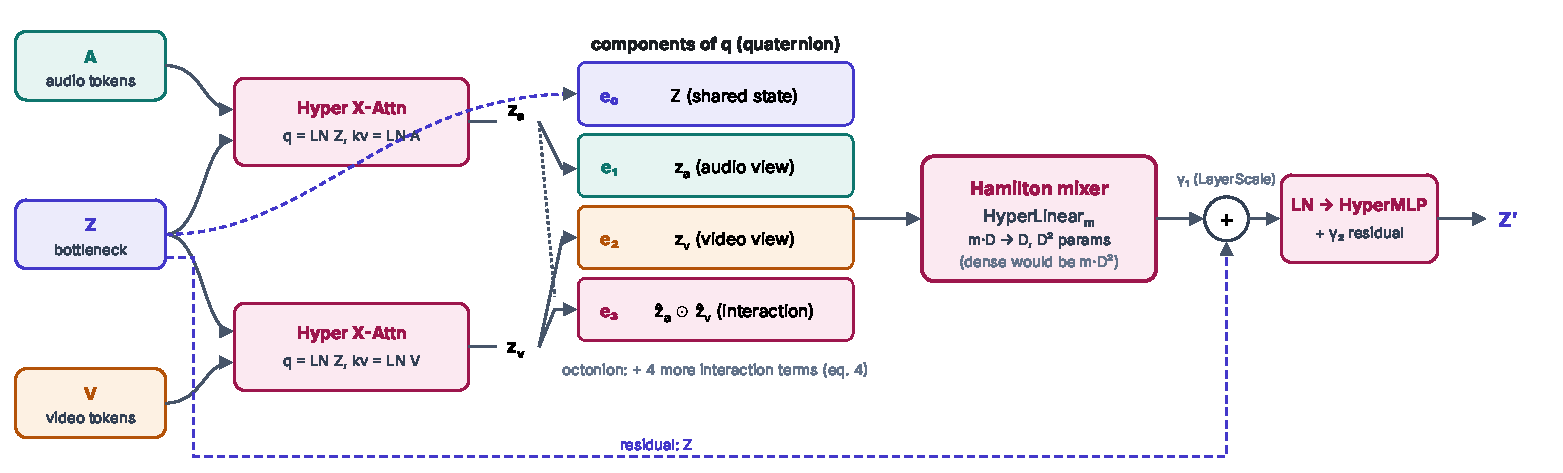
\includegraphics[width=0.9\textwidth]{figures/hcf_block.pdf}
  \caption{Hypercomplex component fusion (HCF), Eqs.~\eqref{eq:xattn}--\eqref{eq:mix}. The modality
  views and their interaction are the components of one quaternion and are mixed by a single
  Hamilton product.}
  \label{fig:hcf}
\end{figure*}

\subsection{Deep-to-early fusion schedule with cross-modal feedback}
\label{sec:schedule}
The set $\mathcal{S}\subseteq\{0,\dots,S-1\}$ selects the stages at which an HCF block is attached:
\begin{equation}
  \mathbf{Z}^{(s+1)} = \begin{cases}\operatorname{HCF}_s\big(\mathbf{Z}^{(s)},\mathbf{A}_s,\mathbf{V}_s\big), & s\in\mathcal{S},\\ \mathbf{Z}^{(s)}, & \text{otherwise,}\end{cases}
  \label{eq:schedule}
\end{equation}
with $\mathbf{Z}^{(0)}=\mathbf{Z}_{\mathrm{init}}$ the learned bottleneck tokens.
Varying $\mathcal{S}$ from $\{S-1\}$ (late fusion) through $\{S-2,S-1\}$ and so on to $\{0,\dots,S-1\}$
gives a controlled \emph{deep-to-early} study of where audio--visual fusion helps. Because the student
backbones are executed stage by stage, the fused state is also fed back into both streams after each
fused stage $s<S-1$:
\begin{equation}
  \mathbf{h}^{m}_s \leftarrow \mathbf{h}^{m}_s\odot\big(1+\tanh(\mathcal{G}^{m}_s\,\bar{\mathbf{z}}^{(s+1)})\big),\quad m\in\{a,v\},
  \label{eq:feedback}
\end{equation}
where $\bar{\mathbf{z}}=\operatorname{mean}_{N_b}(\mathbf{Z})$, the gates
$\mathcal{G}^{m}_s$ are hypercomplex linear maps $\mathbb{R}^{D}\to\mathbb{R}^{C_s}$, and the
product broadcasts over $\Omega$. The gates are \emph{initialised to zero}, so training starts exactly
at the feedback-free model. The network then learns how strongly each modality should condition the
other's later features. This is genuine early fusion, as opposed to fusing independently computed
features.

\subsection{Prediction heads and modality dropout}
\label{sec:heads}
With $\bar{\mathbf{z}}=\operatorname{mean}(\operatorname{LN}\mathbf{Z}^{(S)})$,
$\bar{\mathbf{a}}=\operatorname{mean}(\operatorname{LN}\mathbf{A}_{S-1})$ and
$\bar{\mathbf{v}}=\operatorname{mean}(\operatorname{LN}\mathbf{V}_{S-1})$, the fused and auxiliary logits are
\begin{equation}
\begin{gathered}
  \boldsymbol{\ell} = \mathbf{W}_o\,\operatorname{GELU}\big(\mathcal{H}_n[\bar{\mathbf{z}};\,\mu_a\bar{\mathbf{a}};\,\mu_v\bar{\mathbf{v}}]\big),\\
  \boldsymbol{\ell}^{a} = \mathbf{W}_a\bar{\mathbf{a}},\qquad \boldsymbol{\ell}^{v} = \mathbf{W}_v\bar{\mathbf{v}}.
\end{gathered}
  \label{eq:heads}
\end{equation}
Here $\mu_a,\mu_v\in\{0,1\}$ are per-sample modality masks. During training,
$(\mu_a,\mu_v)=(0,1)$ with probability $p$, $(1,0)$ with probability $p$, and $(1,1)$ otherwise. In the
notation of~\cite{cui2024uffia}, $p_{av}=1-2p$ and $p_a=p_v=p$. The same mask multiplies every fusion
input $\mathbf{A}_s,\mathbf{V}_s$, so a dropped modality is absent everywhere. The auxiliary heads always see
their own modality, which keeps both branches trained regardless of $p$. At test time, forcing
$\mu_a=0$ or $\mu_v=0$ evaluates the model with a missing modality.

\subsection{Training objective and multi-level distillation}
\label{sec:objective}
The supervised loss combines label-smoothed cross-entropy on the fused logits with the two
auxiliary terms:
\begin{equation}
  \mathcal{L}_{\mathrm{sup}} = \operatorname{CE}_{\epsilon}(\boldsymbol{\ell},y)
   + \tfrac{\lambda_{\mathrm{aux}}}{2}\!\!\sum_{m\in\{a,v\}}\!\!\operatorname{CE}_{\epsilon}(\boldsymbol{\ell}^{m},y).
  \label{eq:sup}
\end{equation}
A frozen teacher $g$ with the same output structure (pretrained backbones and HCF fusion) provides
three further signals. At the \emph{logit level}, with temperature $\tau$:
\begin{equation}
  \mathcal{L}_{\mathrm{KD}} = \tau^{2}\,\mathrm{KL}\big(\boldsymbol{\ell}^{g}\,\|\,\boldsymbol{\ell}\big)_{\tau}
   + \tfrac{\lambda_{u}\tau^{2}}{2}\!\!\sum_{m\in\{a,v\}}\!\!\mathrm{KL}\big(\boldsymbol{\ell}^{g,m}\,\|\,\boldsymbol{\ell}^{m}\big)_{\tau},
  \label{eq:kd}
\end{equation}
with $\mathrm{KL}(\mathbf{u}\,\|\,\mathbf{w})_{\tau}=\mathrm{KL}\big(\operatorname{softmax}(\mathbf{u}/\tau)\,\|\,\operatorname{softmax}(\mathbf{w}/\tau)\big)$,
which distils each unimodal head from its counterpart in the teacher. U-FFIA's variant~\cite{cui2024uffia}
softens only the teacher, $\mathrm{KL}(\operatorname{softmax}(\boldsymbol{\ell}^{g}/\tau)\,\|\,\operatorname{softmax}(\boldsymbol{\ell}))$,
and is evaluated as an ablation. At the \emph{embedding level}, small hypercomplex projectors
$\mathcal{P}_k$ align the student's pooled embeddings with the teacher's:
\begin{equation}
  \mathcal{L}_{\mathrm{feat}} = \tfrac{1}{3}\!\!\sum_{k\in\{\bar{\mathbf{z}},\bar{\mathbf{a}},\bar{\mathbf{v}}\}}\!\!
  \big(1-\cos(\mathcal{P}_k(k),\,k^{g})\big).
  \label{eq:feat}
\end{equation}
At the \emph{relation level}~\cite{park2019rkd}, the within-batch similarity structure of the fused
embeddings is matched:
\begin{equation}
  \mathcal{L}_{\mathrm{rel}} = \operatorname{SmoothL1}\big(\mathbf{R}(\bar{\mathbf{z}}_{1:B}),\,\mathbf{R}(\bar{\mathbf{z}}^{g}_{1:B})\big),
  \label{eq:rel}
\end{equation}
where $\mathbf{R}(\mathbf{U})_{ij}=\mathbf{u}_i^{\top}\mathbf{u}_j/(\|\mathbf{u}_i\|\|\mathbf{u}_j\|)$ is the cosine-similarity matrix of a batch of size $B$.
The full objective is
\begin{equation}
  \mathcal{L} = \mathcal{L}_{\mathrm{sup}} + \alpha\,\mathcal{L}_{\mathrm{KD}} + \beta\,\mathcal{L}_{\mathrm{feat}} + \gamma\,\mathcal{L}_{\mathrm{rel}},
  \label{eq:total}
\end{equation}
with $\epsilon=0.1$, $\lambda_{\mathrm{aux}}=0.3$, $\lambda_u=0.5$, $\tau=2$, $\alpha=0.7$, $\beta=1$ and $\gamma=0.5$.
Training proceeds in two stages: the teacher is trained with $\mathcal{L}_{\mathrm{sup}}$ and frozen, then
the student is trained with Eq.~\eqref{eq:total}.

\begin{figure*}[t]
  \centering
  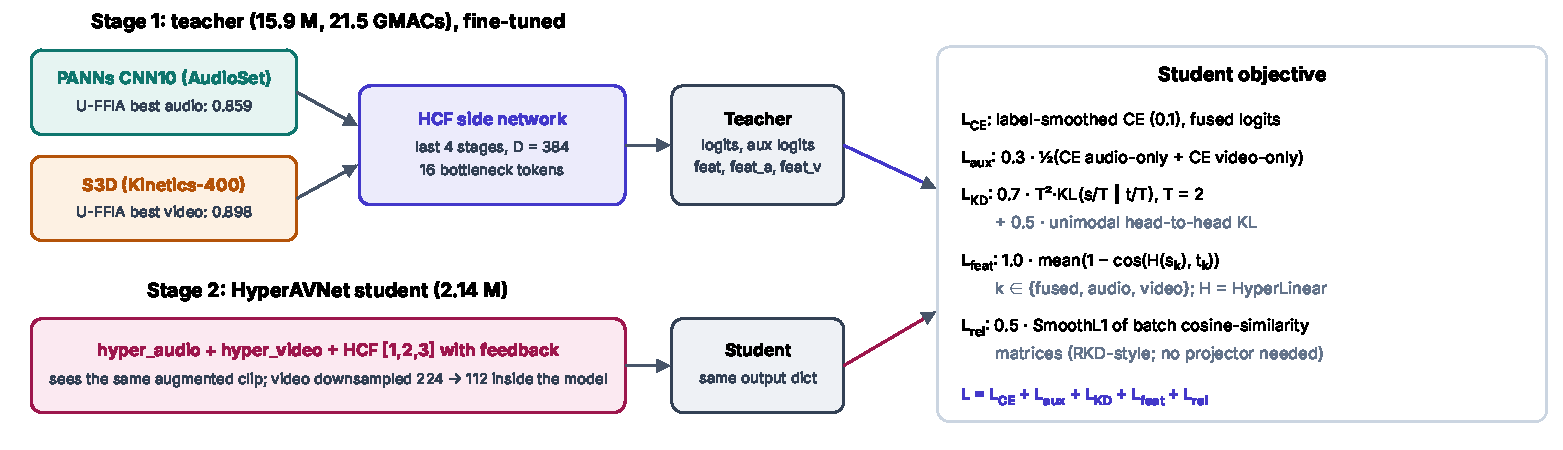
\includegraphics[width=0.92\textwidth]{figures/distillation.pdf}
  \caption{Two-stage training. A teacher built from pretrained audio and video backbones and HCF fusion
  is trained first and frozen. The HyperAVNet student is then trained with the supervised loss plus
  logit-, embedding- and relation-level distillation (Eq.~\eqref{eq:total}).}
  \label{fig:distill}
\end{figure*}

\subsection{Complexity}
\label{sec:complexity}
By Eq.~\eqref{eq:params}, every hypercomplex projection stores $1/n$ of the real parameters. Only the
stems, the depth-wise convolutions, normalisation layers and the final $4$-way classifier stay real.
For the default student ($n=4$), the network has 2.14\,M parameters against 7.88\,M for the identical
real network ($n=1$), and 1.24\,M (octonion) or 0.78\,M (sedenion) for higher algebras. Compute is
1.18\,GMACs per clip for every $n$ (16 frames at $112^{2}$ and 2\,s of audio). The added cost of a
fusion stage is about 0.17\,M parameters and under 0.02\,GMACs.
